\documentclass[authoryear, 12pt,5p, times]{elsarticle}
%\usepackage[hypcap]{caption}
%\geometry{margin=0.95in,top=1.4in,bottom=1.4in}
\geometry{margin=1.1in,top=1.5in,bottom=1.5in}
\usepackage{float}
\usepackage{amsmath}
\usepackage[hidelinks]{hyperref} 
 \usepackage{gensymb}
\usepackage{subcaption}
\usepackage{url}
%\renewcommand\thefootnote{\fnsymbol{\dagger}}
\usepackage[symbol*]{footmisc}
\makeatletter
\newcommand{\rpm}{\raisebox{.3ex}{$\scriptstyle\pm$}}
\begin{document}
%\footnote{This is a footnote}
\begin{frontmatter}
\title{Introductory Experiments and Linear Circuits I}
\author{\today \quad \\Jung Lin (Doris) Lee [Lab Partner: Leah Tom]\\Prof. William Holzapfel, GSI Thomas Darlington, Thomas Mittiga, John Groh,  \\Victoria Xu, Jonathan Ma, Francisco Monsalve, Xiaofei Zhou}
	 
\end{frontmatter}
   %key objective, method, principle conclusion 
%	  In our experimental setup, photons emmited by an LED light source is regestered by the PMT as a timestamp for every photon detection. By increasing the brightness of the light source, we found that photon arrival rates increase. Analysis on a single dataset shows that as the the number of events in an experiment (N) increases, the sample mean($\bar{x}$) converges to the theoretical mean($\mu$).  The fluctuation around this value of $\mu$ falls off as with 1/$\sqrt{N}$, so increasing N can results in more reliable experimental results. However, systematic effects can not be eliminated by such methods. We instead mitigate the afterpulsing effect by vetoing events that occurred immediately after another. The processed data results in a histogram that align very closely to exponential distribution. In addition, binned data for a fixed time interval also matches closely with the Poisson distribution. Finally, we can obtain the sample mean parameter for this  experiment by fitting the histogram to the Poisson distribution.  

\section*{Introduction\label{intro}}
\indent 
Digital Multimeter (DMM), oscilloscope, and signal generator are essential tools used to obtain measurements in experimental physics. In this lab, we use these measurements further our understanding of linear circuits.  Linear circuits, obeying the simple Ohm's law, are the basis to understanding the workings of more complex circuitry. Using the powerful Thevenen's theorem,  complex arrangements of linear components can be regarded as a black box with a single resistor and voltage source.  \par We are then introduced to the notion of impedance, which generalizes methods used for linear circuits to AC circuits. AC-powered devices are ubiquitous not only in household applications, but also in experimental physics laboratories. Throughout the lab exercises, we compute the errors associated with each measurement, as numerical results are meaningless if they are not presented with an estimate of the uncertainty.
 \par  In this report, we present the methods used to conduct the series of experiments in Lab 1 and the obtained measurement results. In part one, I will detail the experimental methods and the usage of various instrumentation that were employed to take the data.  Then, part \ref{part2} focuses on the analysis of circuits with linear components. 
\section{Part I: Introductory Experiments }
% \subsection{Keithley 2110 Digital Multimeter3 (DMM)}
%- uncertainty
%The range should be adjusted  suitable range within --- for each measurement , within order of magnitude. \footnote{Too large a range will result in the error ``OVLRD" (overload) and too low will cause ---}
\subsection*{BSC Laboratory Breadboard Box}
\begin{figure}[h!]
\center
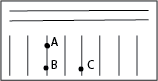
\includegraphics[width=0.3\textwidth]{figure/breadboard}
\caption{We put jumper wires connecting the A and B, B and C separately and measure the resistance across them.}
\label{breadboard}
\end{figure}
\paragraph{\textbf{1.1}}
The breadboard is a device suitable for rapid-protoyping circuits, without long chemical etching process of the PCB.  As shown in Fig.\ref{breadboard} , it is horizontally connected along the longer edge for the two top and bottom buses, which often serves as a power line for the input voltage and grounding terminals. We measured the resistance across A and B as 0.16 $\Omega$ and across B and C as ``overload".  These result make sense because since B and C is not connected, the resistance is almost infinite, and is therefore not registered on the DMM. Likewise, since A and B are connected, there is minimal resistance between them.
\paragraph{\textbf{1.2}}
\par a)  We connect the 12V to -12V to set up the +24V potential difference across the two terminals. Then we connect the -12 to ground to prevent the common to ``float", as shown in Fig. \ref{24}
\begin{figure}[h!]
\center
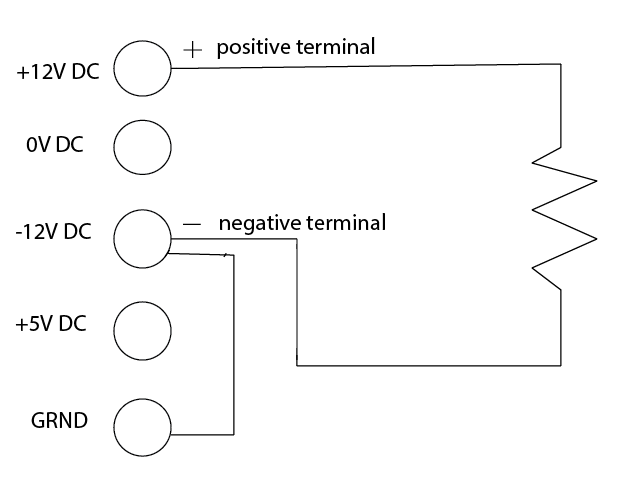
\includegraphics[width=0.5\textwidth]{figure/parta}
\caption{Setup for +24V relative to ground.}
\label{24}
\end{figure}
\par  b)	Again, we connect the 12V to -12V to set up the +24V potential difference across the two terminals. To get the flip the sign of the voltage reading on the DMM, we connect the +12V terminal to ground.
\par  c) Connecting the negative  terminal to 0V and the postive terminal to -12V, then connect 0V to ground as usual, we obtain the 12V reading. 
\par  d)	Again, we have the same setup as c) but the polarities are reversed, the positive is connected to 0V and the negative to the 0V instead.
\par  e)	To again prevent the ``floating" of common and ground, we connect -12V to ground and then connect the negative terminal to -12V and the positive terminal 5V to generate the 17V potential difference as predicted.
\paragraph{\textbf{1.3}} 
The readings between the 12 output and the 5V supply ground fluctuates around 0V. The reasoning behind this result is that the 12V terminal and 0V pair only supply a 12V potential difference with respect to ground. However, the common and the ground is not necessarily at the same potential.  If the common and ground is not connected, we must consider the left and right voltage terminals in Fig. \ref{ground_common} as distinct. Therefore, connecting the 12V and 5V terminal essentially brings them both to equipotential, resulting in a potential difference of $\approx$  0V.
\begin{figure}[h!]
\center
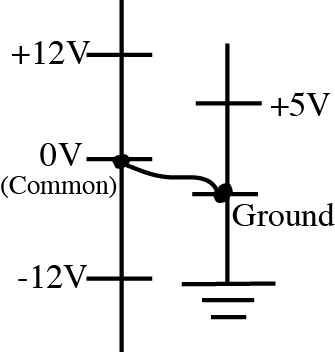
\includegraphics[width=0.25\textwidth]{figure/ground_common}
\caption{By connecting the ground to the common, we can set both the 12V and the 5V with respect to ground, thereby creating the 17V output voltage.}
\label{ground_common}
\end{figure}

%%%%%%%%%%%%%%%%%%%%%%%%%%%%%%%%%%%%%%%
\paragraph{\textbf{1.4}} \label{1_4}
We build the circuit as shown in \ref{voltage_divider}. To compute the voltage at point A , we first compute the current through R1 and R2: 
\begin{equation}
I = \frac{V}{R_{1} + R_{2}}
\label{I} 
\end{equation}
Then, we determine the voltage at point A through Ohm's law:
\begin{equation}
 V_{A} = I R_{2} = \Bigg(\frac{R_{2}}{R_{1} + R_{2}}\Bigg)V
 \label{voltage_divider_eq}
\end{equation}
%%%%%%%%%%%%%%%%%%%%%%%%%%%%%%%%%%%%%%%
\paragraph{\textbf{1.5}} \label{1_5}
Since the resistors are arranged in series as shown in Fig.\ref{voltage_divider}, the current through each resistor should be the same.  
\begin{equation}
I=\frac{V}{R_{eq}}=\frac{V}{R_1+R_2}=\frac{24V}{480k\Omega
}= 5.0\times10^{-5}A 
\end{equation}
%%%%%%%%%%%%%%%%%%%%%%%%%%%%%%%%%%%%%%%%
\textbf{1.1.6} % change the number of the equation referenced based on final report numbering
Using Eq.\ref{I}, we plug in the nominal values:
\[ R_{1} = 470 k\Omega, R_{2} = 10k\Omega, V = 24V \]
\begin{equation*}
V_{A} = \frac{10k\Omega}{(470+10)k\Omega}\times 24V \\
= 0.5 V
\end{equation*}
%%%%%%%%%%%%%%%%%%%%%%%%%%%%%%%%%%%%%%%%
\paragraph{\textbf{1.7}} 
\begin{figure}[h!]
\center
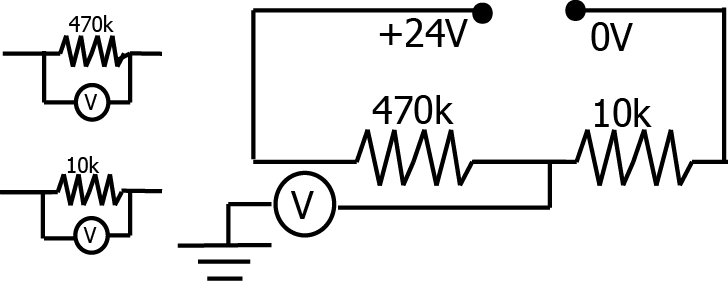
\includegraphics[width=0.5\textwidth]{figure/1_7_setup}
%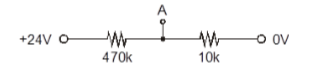
\includegraphics[width=0.25\textwidth]{figure/d_voltage_divider}
\caption{The voltage divider setup for this experiment.}
\label{voltage_divider}
\end{figure}
a) Depending on the DMM setup, it can act as a voltmeter or ammeter. To measure the current through a 10k$\Omega$ resistor, we need to connect the DMM in parlalle lwith the 10k$\Omega$ resistor as shown in the bottom left of Fig.\ref{voltage_divider}.
Then, using Ohm's law we can compute the current flowing through the 10k$\Omega$ resistor: 
\begin{equation}
I = \frac{V}{R}=\frac{0.510V}{10k\Omega}=5.1\times 10^-5 A
\label{current}
\end{equation}
which is approximately the same as predicted in \ref{1_5}. Alternatively, we can also connect the DMM in series with the resistor as shown in the top right figure of Fig. \ref{voltage_divider}  to measure the current directly, and this yields the same current value as computed in Eq.\ref{current}.\footnote{Note that the ground and sensing probes need to be plugged into a different set of holes instead of the two terminals plugged in for the voltage measurement. Both the upper pairs will work but the upper left pairs  gives a more precise reading.} 
\\
b)  We connected the DMM across the  470k$\Omega$ resistor as show in the lower left figure in Fig. \ref{voltage_divider} and obtained a reading of 24.079V, with the range set as 10V. Using Eq. \ref{accuracy1_7}, we compute the actual reading range as 24.079V $\pm $3.29mV:
\begin{equation}
0.012\% \times 24.079V+0.004\%\times10V=3.28948mV
\label{accuracy1_7}
\end{equation}
%%%%%%%%%%%%%%%%%%%%%%%%%%%%%%%%%%%%%%%%
\paragraph{\textbf{1.8}} 
The gold band indicates that both resistors have tolerances of about 5\%. Using the DMM, we find that the actual value of the \(10k\Omega\) resistor is \(9.89k\Omega \) and  \(470k\Omega\) one is \(465.6k\Omega\). The actual input voltage measured across the terminals are 24.5V, which is 2.08\% different from its nominal value of 24V. For the \(10k\Omega \) resistor, the percentage difference between its nominal and actual value is 1.1\%. Likewise, the \(470k\Omega\) resistor differs  0.936 \%  from its actual. Both the resistors and the voltage sources agree within the specified tolerances of 5\%.   

%%%%%%%%%%%%%%%%%%%%%%%%%%%%%%%%%%%%%%%%
\paragraph{\textbf{1.9}} 
The current through each resistor is: 
\begin{equation}
I = \frac{24.589V}{(465.6+9.89)k\Omega} = 0.0517mA
\end{equation}
There is a 0.17\% deviation from the nominal values computed in \ref{1_5}.
Using Eq.\ref{voltage_divider_eq}, the voltage at point A is computed as: 
\begin{equation}
V_A= \frac{24.589V \times 9.89k\Omega}{(465.6+989)k\Omega} = 0.5114V
\end{equation}
Comparing this result with nominal values from question 1.6, there is a 1.14\% error.
%%%%%%%%%%%%%%%%%%%%%%%%%%%%%%%%%%%%%%%%
\paragraph{\textbf{1.10}} 
We measured $V_A$ as 0.51085V, using the range setted on the DMM  as 1V. We can therefore compute the uncertainty of the reading as:
\\
\( (\frac{0.012}{100} \times 0.51085) + (\frac{0.04}{100} \times 1)
 = 4 \times 10^{-4} V  \) \\ \\
We can thereby quote our measurement as \(V_{A} = 0.51V \pm 40mV\). The discrepancy between our actual reading and the nominal value (\( 0.51 - 0.5 = 0.01V \)) can not be entirely accounted for by this measurement uncertainty, which means that there must be other error terms not accounted in the uncertainty calculation.
%%%%%%%%%%%%%%%%%%%%%%%%%%%%%%%%%%%%%%%%
\paragraph{\textbf{1.11}}
The current through $R_1$ is computed by :
\begin{equation}
I_1 = \frac{24.072V}{ 470k\Omega} = 5.1217\times10^-5A
\end{equation}
The current through $R_2$ is computed by:
\begin{equation}
I_2 = \frac{0.51079V}{ 9.89k\Omega} = 5.1617\times10^-5A
\end{equation}
We connect the ammeter in series and change the prong on the DMM to the bottom two terminals and measured the current directly as 0.0030 mA$\pm 3.64\times10^{-7} mA $.  \footnote{Computed by Eq.\ref{accuracy1_7}}
%%%%%%%%%%%%%%%%%%%%%%%%%%%%%%%%%%%%%%%%
\paragraph{\textbf{1.12}}
\par a) The power dissipated by a resistor is computed by $V^2/R$. Using nominal values for the resistor, the power dissipated by the \(10 k\Omega\) resistor is \(2.5 \times 10^{-5} W \). Similarly, the power dissipated by \(470 k\Omega \) resistor is \(  1.18 \times 10^{-3} W\)
Both of these resistors have power rating of 0.25W (``quarter-watt"), they are both dissipating power within this limit. 
\par b) Given that the  voltage supply and ratio of resistor ,  in order to increase overall power to approach the maximum power, I would decrease the resistor values, since  P=$V^2/R$ (i.e. P \(\propto \frac{1}{R} \)). 
\par c) The \(10k\Omega\) resistor would reach its maximum power rating first since the voltage across each resistor is constant, therefore the resistor with a smaller value reaches the threshold value of resistance first since \(P \propto \frac{1}{R}\).  
\par d) Set the power to 0.25W :
\begin{equation*}
P = I^2R = (0.05mA)^2R=0.25W
\end{equation*}
and rearrange to solve for R, we get \(R = 10000k\Omega\). So we need to make the resistor approximately 200 times smaller. For the second resistor, we need to make the resistor 10000 times larger.
\par  e)  $10000k\Omega$ is not a common value for a resistor. At this value, the resistor is almost an insulator. We can build this by putting may resistors in series, but require many added together so  would be difficult to build.%We can arrange several resistors in parallel to decrease its effective resistance, but in practice, we would require a lot of parallel resistor so this will probably be hard to build.
\subsection*{Frequency and time measurements}
%%%%%%%%%%%%%%%%%%%%%%%%%%%%%%%%%%%%%%%%
\paragraph{\textbf{1.17}}
a) We measured the voltage measurement as 5.0488V and the error on the measurement is computed by: 
\begin{equation*}
0.012\%(5.0488V)+0.004\%(10V) = 1.0059V
\end{equation*}
\par b) We adjusted the settings of the oscilloscope to add the  measurement of the mean and amplitude and obtained a reading of 4.984V and 240.0 mV respectively. Since our signal is a flat line on a V-t graph, the fluctuation on the y axes informs us about how the voltage changes in time. The amplitude is the variance on the averaged voltage value that we obtained, and therefore serves as an estimate for the error our voltage measurement. 
\par
c) We find that as we decrease the voltage per division, our amplitude (estimated error) also decreases. The more refined division of the voltage values scale results in greater precision of the measurement, analogous to how the range of our DMM must be adjusted to minimize the uncertainty of the  measurement.
\par
d) The best scope setting is the 1V/div since yields the smallest variance. \footnote{Any settings for 1V/div  or below is not accurate enough  for the oscilloscope to conduct a measurement since the time averaging window does not contain all  of the signal . For example, the 500mV/div setting yields a variance of $>$2.56V, which is over 50\% error relative to the actual value.}

%%%%%%%%%%%%%%%%%%%%%%%%%%%%%%%%%%%%%%%%
\paragraph{\textbf{1.18}} 
\par a) By switching the oscilloscope's ``coupling" option from DC to AC, we see rapidly fluctuating voltages. This setting effectively filters out all the DC signal (voltages that are constant in time) and keep only the signal that alternate in time. 
\par  b) When we zoomed in the horizontal axes time scale, the AC component of the output rapidly fluctuates in time, is noise-like, and has a high frequency. 
%%%%%%%%%%%%%%%%%%%%%%%%%%%%%%%%%%%%%%%%
\paragraph{\textbf{1.19}} 
The root mean square voltage ($V_{rms}$)is often given as a useful quantity for finding the power. The $V_{rms}$ is defined by the root of the time-averaged,squared voltage as:
\begin{equation}
V_{rms} = \sqrt{\frac{1}{T}\int_0^{t_0} V_s(t) ^2 dt} 
\end{equation}
$\text{Let us define} V_0 = \text{Amplitude}$,\footnote{The ``amplitude" measurement option of the oscilloscope defines its readings as 2$V_0$, a value close to the $V_{pp}$ reading.}$V_{pp} =  $Peak-to-peak voltage= 2$V_0$ , $V_s$= signal's voltage. 
\par  a) For a sine wave signal, the $V_{rms}$ is computed by: 
\begin{align}
V_{rms} = V_0\sqrt{ \frac{1}{2\pi}\int_0^{2\pi}sin^2 x}= \frac{V_0}{\sqrt{2}}
\end{align}
\par b) For a triangular wave signal, we can simply compute over 1/4 of its period, since the area under the signal in that interval is the same (i.e. power and $V_{rms}$): 
\begin{align}
V_{rms} = \sqrt{ \frac{4}{T}\int_0^{\frac{\pi}{2\omega}}\Bigg(\frac{V}{\pi/2\omega}\Bigg)^2 xdx}=\frac{V_0}{\sqrt{3}}
\end{align}
\par c) Geometrically, we can see that the $V_{rms}$ of a square wave signal is equal to its $V_0$.
We measure the V$_0 $, V$_{pp}$, V$_{rms}$ of a input signal on the oscilloscope, as shown in Table \ref{Vrms_table}. 
%\footnote{Uncertainty computed by Eq.\ref{accuracy1_7}}.
\begin{table}
    \begin{tabular}{l|l|l|l}
    Type       & V$_0 $(mV) & V$_{pp} (V)$ & V$_{rms}(mV)$ \\ \hline
    sine       & 496   & 1.02      & 351        \\
    square     & 490   & 1.68      & 490        \\
    triangular & 510    & 1.04      & 283        \\
    \end{tabular}
\caption{Experimental values for oscilloscope measurements. The $V_{rms}$ computed in parts a, b, and c is 361, 485, 255 mV, respectively, which is within 10\% of experimentally obtained values.}
    \label{Vrms_table}
\end{table} 

%%%%%%%%%%%%%%%%%%%%%%%%%%%%%%%%%%%%%%%%
\paragraph{\textbf{1.20}} 
Using a sine wave of $V_{pp}$ =1 and variable frequency, we measure the RMS voltage as plotted in Fig.\ref{1_20}. Both the plots for question a and b are superimposed for visual comparison of finding the frequency range.\begin{figure}[h!]
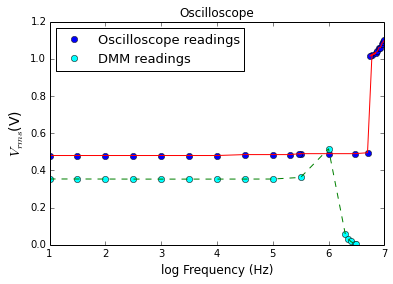
\includegraphics[width=0.5\textwidth]{figure/1_20}
\caption{Root mean square voltage measured by the oscilloscope and by the DMM.}
\label{1_20}
\end{figure}  
\par The reason why we take data by varying frequency geometrically rather than arithmetically is because the comparison can be better shown if the values are plotted with the x axes logged. In that case, the geometric increments of frequency will appear as evenly spaced data points, whereas a choice of a arithmetic frequency values would make the data points seem cramped up in the lower frequency values. By examining these two graph, the DMM and the oscilloscope values agree within 5\% over the frequency range below 1MHz. According to the Keithley 2100 Data Sheet, the DMM performs optimally from 3Hz to 300kHz, which agrees with the results that we see in Fig.\ref{1_20}.
%%%%%%%%%%%%%%%%%%%%%%%%%%%%%%%%%%%%%%%%
\paragraph{\textbf{1.21}} 
\begin{figure*}[t]
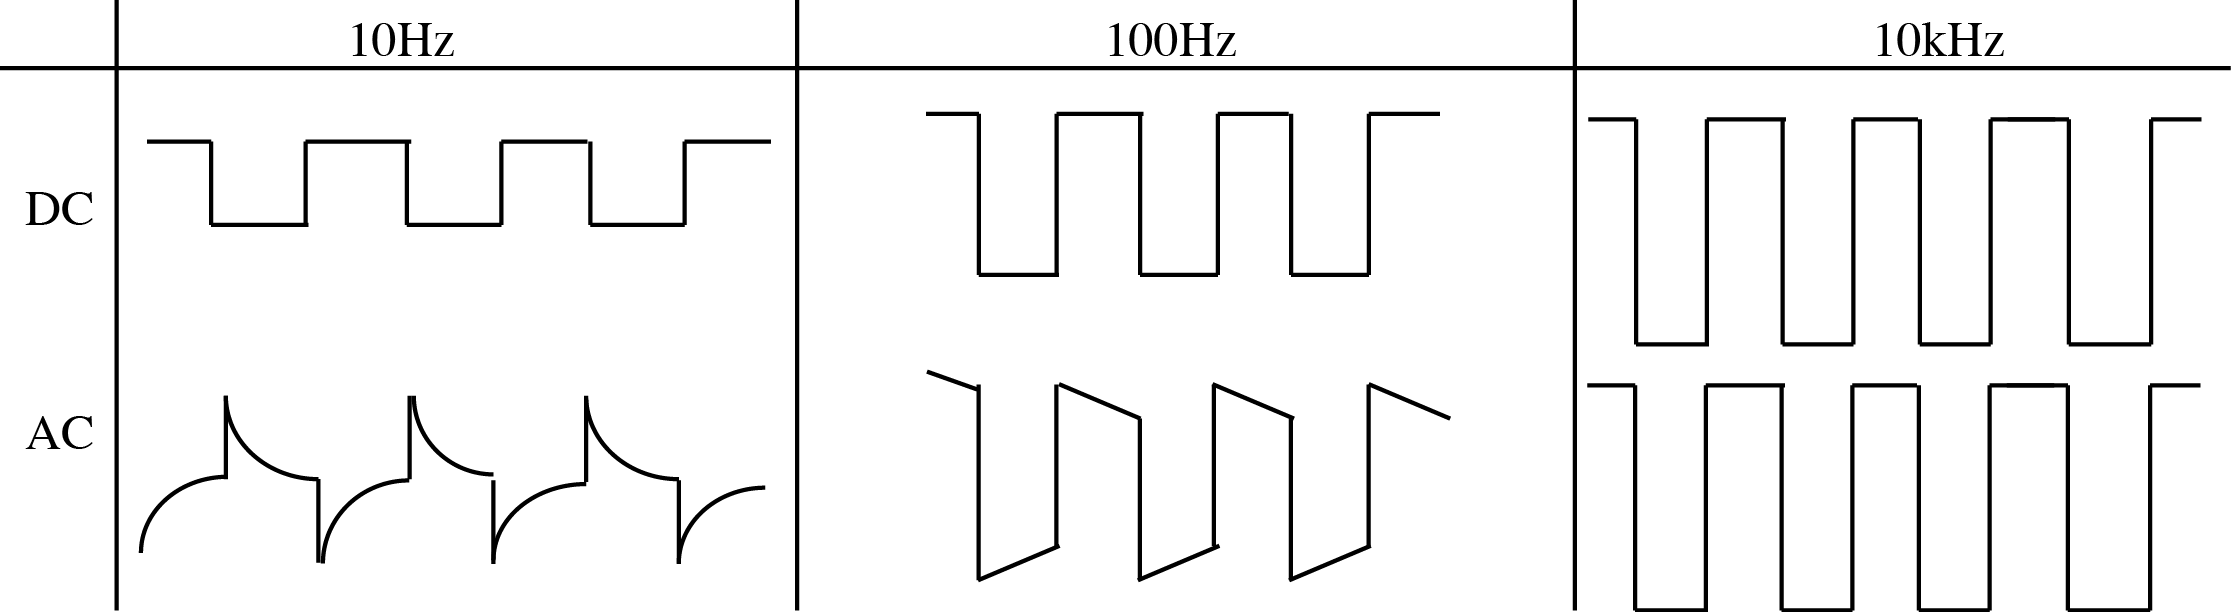
\includegraphics[width=\textwidth]{figure/ACweird}
\caption{At low frequencies, the AC scope traces on the oscilloscope experience distortion.}
\label{AC_weird}
\end{figure*}
The AC setting on the oscilloscope subtracts off the average value from the DC signal. This average is taken over some fixed time interval. So by decreasing the frequency, there will be fewer cycles in the same amount of sampling time, therefore the computed average will be less accurate. Subtracting off such a value yields the sloped wedges seen in 10 and 100 Hz  AC scope traces, as shown in Fig. \ref{AC_weird}.\footnote{Note that the 50$\Omega$ terminator introduces noise to to the scope reading. Therefore, we replaced the terminator component with the ``High Z" setting load on the signal generator.}
\section{Part II: Linear Circuits}\label{part2}
\subsection*{Thévenin Analysis}
%%%%%%%%%%%%%%%%%%%%%%%%%%%%%%%%%%%%%%%%%%
\paragraph{\textbf{2.1}}
\begin{figure}[h!]
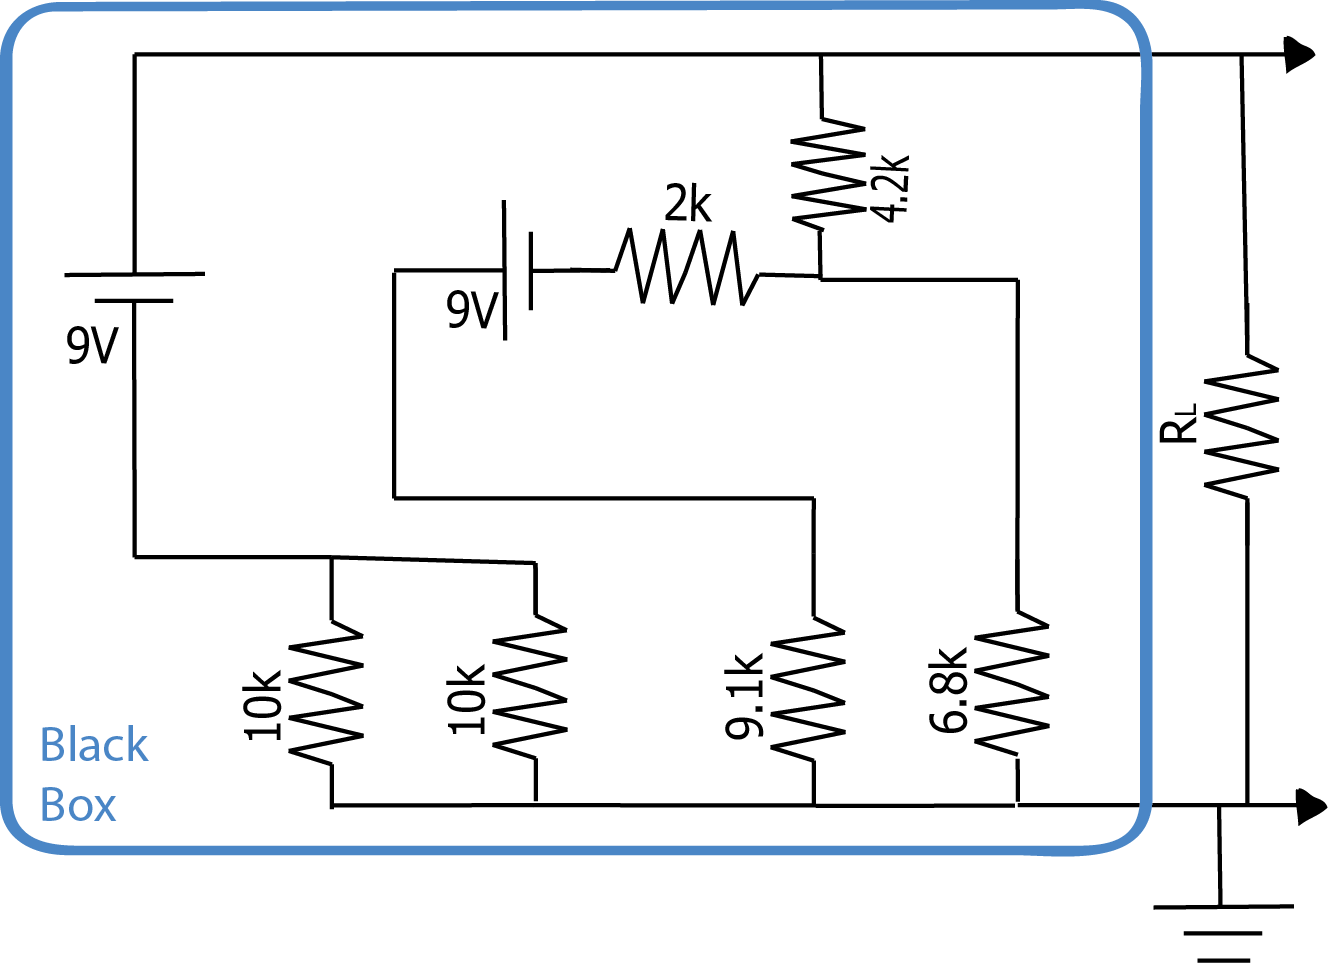
\includegraphics[width=200pt]{figure/thev_setup}
\caption{Using the resistor color chart, we decoded the resistor values  in the black box and computed the $V_{eq}$ and $R_{eq}$.}
\label{thev_setup}
\end{figure}
Since the battery is in parallel in the Thevenin circuit, the equivalent voltage is 9V. By decomposing the complicated Thevenin circuit into series and parallel parts, we can compute the equivalent resistance as 3.1367 k$\Omega$. Using Thevenin's theorem, since the components of the black box are all linear, we can simply treat everything in the Thevenin circuit (denoted by the blue box in Fig\ref{thev_setup}) as a single voltage source of $V_{eq}$ and resistor with $R_{eq}$. We used the measured the open-circuit voltage 4.1033V and the short circuit 1.2473mA to compute the Thevenin resistance:
\begin{equation}
R_{thev} = {V_{open}}{I_{short}}= \frac{4.1033V}{1.2473mA}=3.2897k\Omega
\end{equation}
which is within 5\% difference from the $R_{thev}$ computed from the nominal resistance values of the black box.
\begin{figure}[h!]
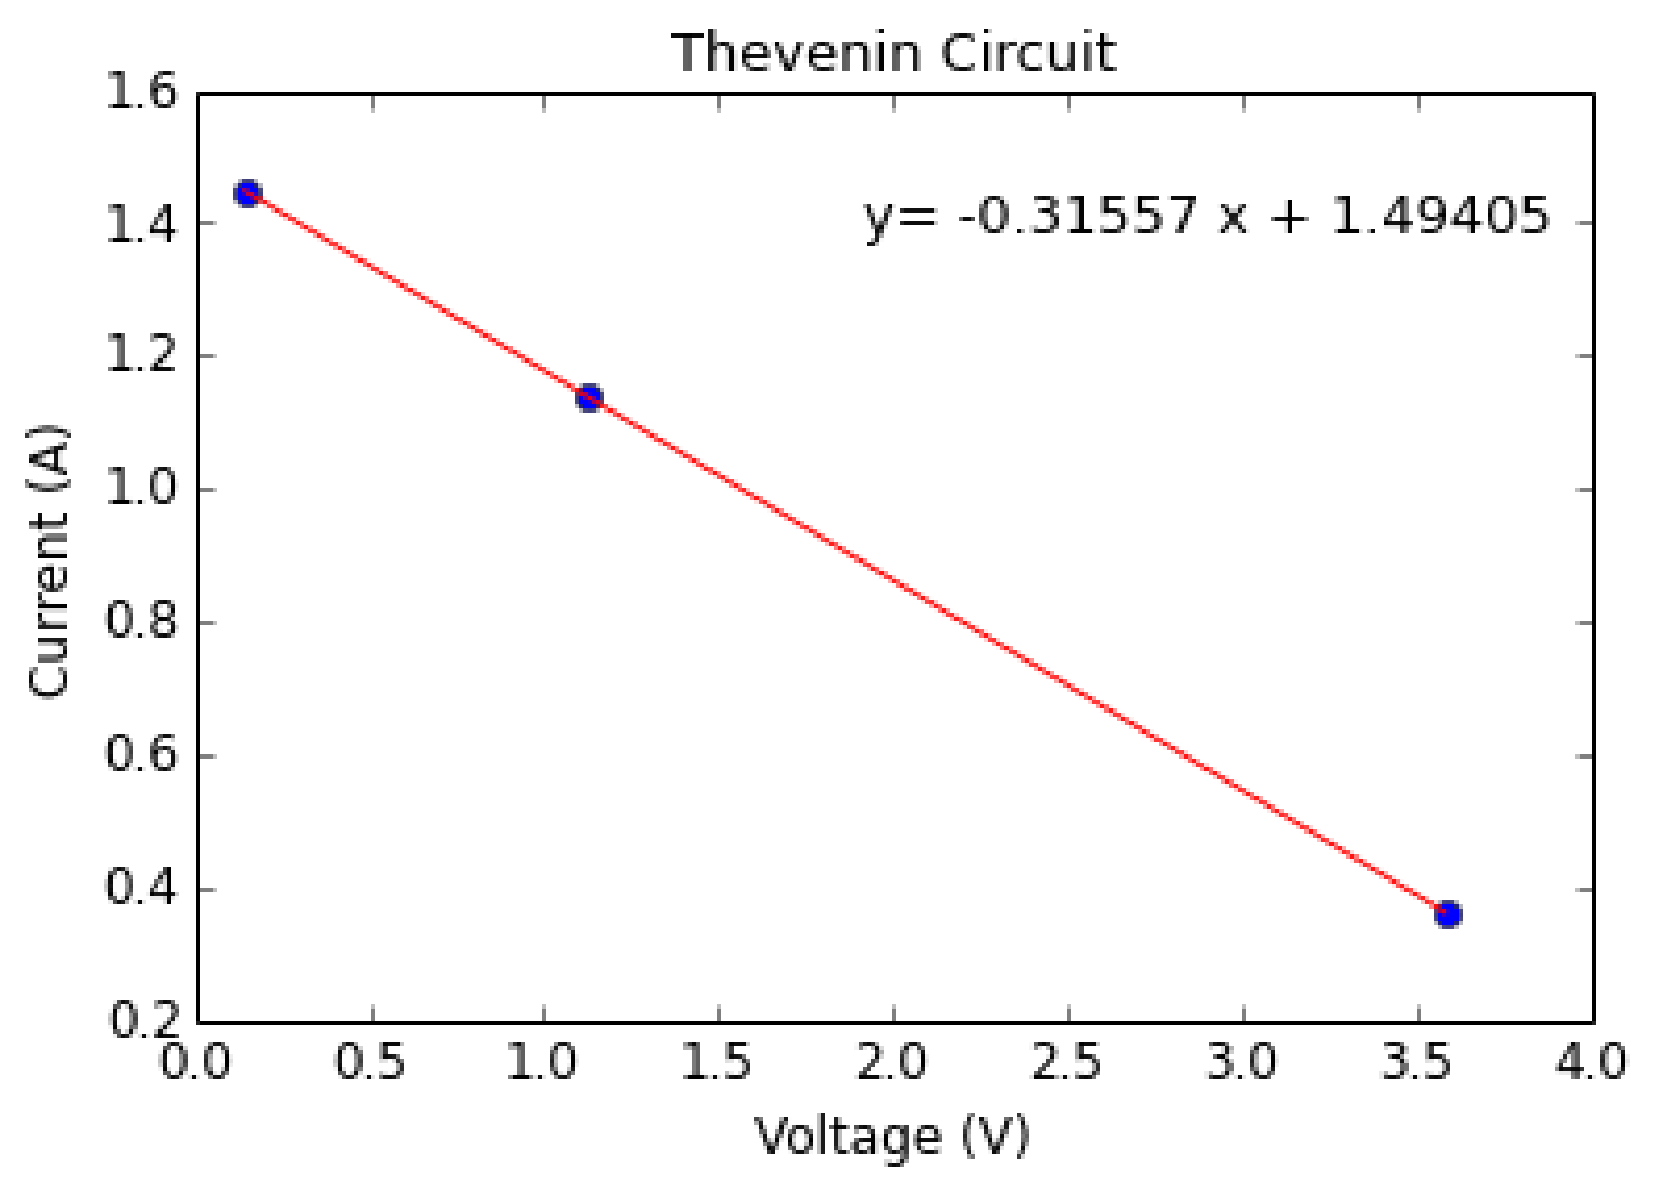
\includegraphics[width=200pt]{figure/thevenin}
%\caption{A straight-line fit through the data points for different values of load resistors shows that the output impedance is 0.32 $\Omega$.}
%\caption{The measurement of ------ slope is ---- , different values of load resistors. The measurement setup is illustrated in Fig. (REF!!).}
\caption{These voltages measurement accurately predict the trend that   as the load resistance increases, the current through the resistor decreases.}
\label{thevenin_plot}
\end{figure}
By shorting the battery with a jumper wire, we effectively bring the battery's terminals to equipotential, causing the output voltage to be 0V. The DMM measurement of resistance across the two terminals is 6.7k$\Omega$ which is 3.35k$\Omega\pm 0.442\Omega$.\footnote{Determined  by Eq.\ref{accuracy1_7} for the measurement and range of 1k$\Omega$. The computed $R_{thev}$ lies in this range.}
%%%%%%%%%%%%%%%%%%%%%%%%%%%%%%%%%%%%%%%%%%
\paragraph{\textbf{2.2}}
 We set up the oscilloscope to 50mV/div and 5ms/div and connected a mini-grabber clip to it.
a) When we touched the end of the red mini-grabber lead, we saw a signal of about 60Hz on the oscilloscope. We eliminated the possibility of the human heart beat since it This signal is due to the frequency that is being outputted by the wall sockets (the frequency is roughly 60Hz). However, it is not from the wall sockets that we radiate out this frequency. Electronic appliances such as the computer monitor radiate out EM waves at that frequency and our body transfers this signal when we touch the conducting part of the mini-grabber, the signal is picked up and we therefore see a 60 Hz sinusoidal signal on the oscilloscope.
\par b) Pinching the red insulation of the minigrabber clip does not result in a signal on the screen of the scope. This is because the minigrabber is well insulated and thus no signal gets through.
\par c) Pinching the BNC cable also does not result in a signal for the same reason as part b). The BNC cable is well insulated and thus prevents the intrusion of different waveforms. However, if you distort the BNC cable by bending it at a sharp angle then the path that the wave is travelling through is also distorted momentarily, causing the wave to be reflected, but after a few seconds the signal resumes its original shape.

d) When we short the mini-grabber signal and ground leads with a four-foot long insulated wire, we do see a signal. This signal seems to be there because the loop of the wire acts as an antenna that is able to pick up noise. The noise the antenna picks up is ambient waves being radiated by our body. The scope trace looks like the following graph:
\begin{figure}[h!]
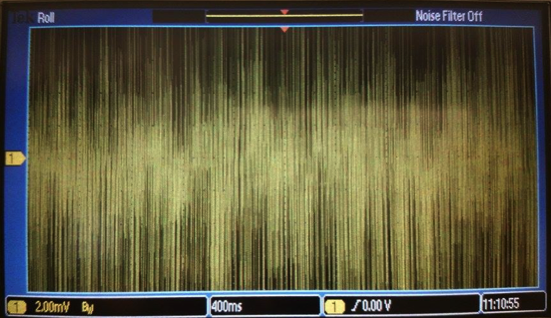
\includegraphics[width=0.5\textwidth]{figure/trace_2_2e}
\label{trace2.2e}
\caption{The oscilloscope traces illustrates the noise detected by the antenna from waves in the environment.}
\end{figure}


%%%%%%%%%%%%%%%%%%%%%%%%%%%%%%%%%%%%%%%%%%
\paragraph{\textbf{2.3}}
Here, we treat the oscilloscope as a black box of unknown impedance.  We substituted different resistors in the circuit shown in  Fig.\ref{Z_input}, and measured the input voltage. Using Eq.\ref{I_input}, we compute the input current as plotted in Fig. \ref{Z_input_plots}
\begin{equation}
I_{in} =\frac{V_{ext}-V_{in}}{R}
\label{I_input}
\end{equation}
From Eq.\ref{Z_in}, we see that the value of the slope is equivalent to the input impedance. A linear regression on the data results in a slope of 0.1978 M$\Omega\pm 8.24\times10^{-5}\Omega$. 
\begin{equation}
Z_{in}=\frac{V_{in}}{V_{ext}-V_{in}}R =\frac{V_{in}}{I_{in}}
\label{Z_in}
\end{equation}This result of a large input impedance makes sense since a larger impedance prevents the current to flow through easily, so that the oscilloscope does not perturb the circuit when conducting measurements.
\begin{figure}[h!]
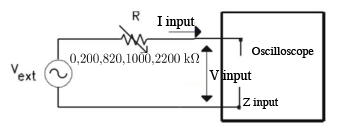
\includegraphics[width=0.5\textwidth]{figure/Z_input}
\label{Z_input}
\caption{The circuit setup to find the $Z_{input}$ of the oscilloscope.}
\end{figure}
\begin{figure}[h!]
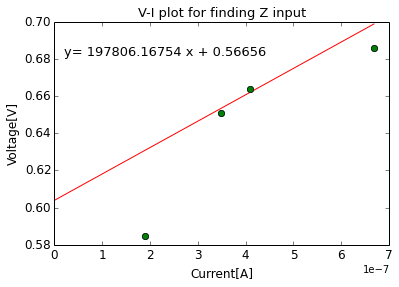
\includegraphics[width=0.5\textwidth]{figure/Z_input_plot}
\caption{The uncertainty is computed according to Eq.\ref{accuracy1_7}, with range of 0.001V and 0.1mV for the last measurement. Since the error is on the order of magnitude of $10^{-5}$, the error bar plotted on this graph can not be seen unless zoomed in. }
\label{Z_input_plots}
\end{figure}
%%%%%%%%%%%%%%%%%%%%%%%%%%%%%%%%%%%%%%%%%%
\paragraph{\textbf{2.4}}
We set up the scope probe as shown in Fig.\ref{2_4_setup}, then measure the voltage as we vary the resistance. Here, we again treat the oscilloscope as a black box. 
\begin{figure}[h!]
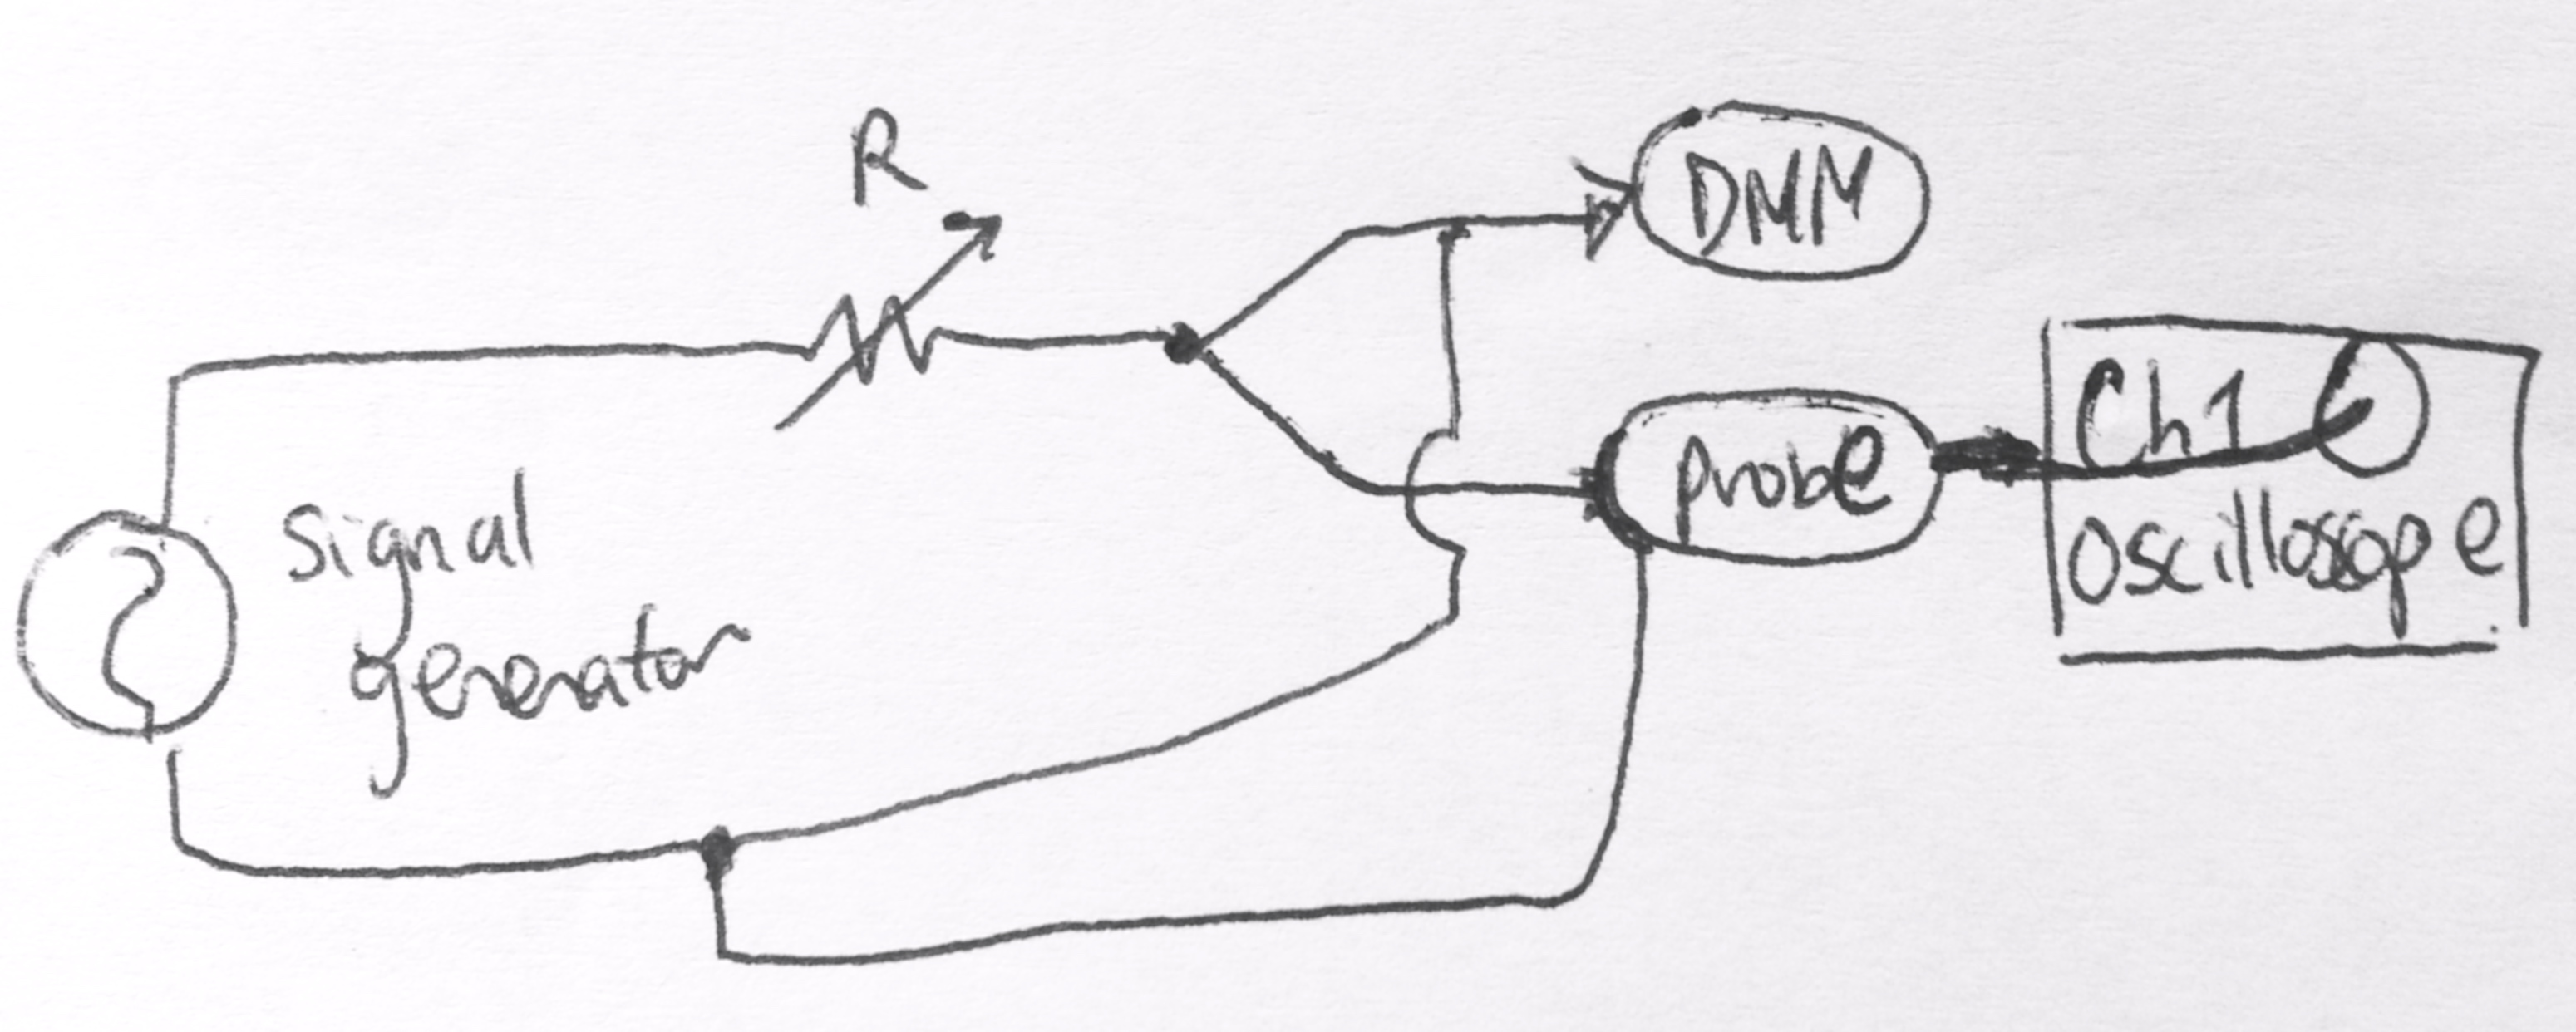
\includegraphics[width=0.5\textwidth]{figure/2_4_setup}
\caption{The circuit setup used to measure the voltage as we insert different values of resistors (0$\Omega$,200k$\Omega$,470k$\Omega$,820k$\Omega$, 1M$\Omega$,2.2M$\Omega$).}
\label{2_4_setup}
\end{figure}
 The range in the DMM setting while measuring \(V_{in}\) is 0.00001V, we can use this to compute the uncertainty of each measurement using \ref{accuracy1_7}, which comes out to an error on the order of magnitude of $10^{-5}$ V. Using the measured  input voltage and the nominal external resistance, we can calculate the input current by : 
\begin{equation}
I_{in} = \frac{V_{ext} - V_{in}}{R}
\end{equation}
Since input impedance is defined as \(Z_{in} = \frac{V_{in}}{V_{ext} - V_{in}}R\), we can plot a graph of input voltage against input current and calculate the slope to find the input impedance. As seen on Figure \ref{2_4_plot}, a linear fit through this graph yields a slope of 447008.763\(\Omega\). This input impedance result is more than doubled the input impedance based on the DMM readings.  This tells us that the measurement of the input voltage by the scope probe is more accurate since it yields the result for the larger impedance (i.e. the measurement approaches the limit of the ideal , infinite resistance of the voltmeter).
\begin{figure}[h!]
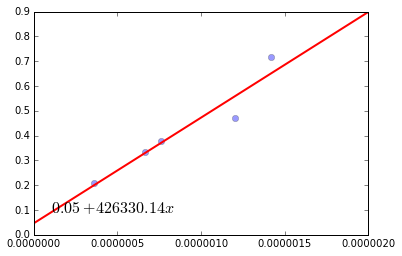
\includegraphics[width=0.5\textwidth]{figure/1-2-4-input-impedance} 
\caption{Linear regression on the datapoint yields the slope as the input impedance of the oscilloscope.}
\label{Input_Impedance_probescope}
\end{figure}
%%%%%%%%%%%%%%%%%%%%%%%%%%%%%%%%%%%%%%%%%%
\paragraph{\textbf{2.5}}
 Treating the signal generator as the black box, as shown in \ref{Z_output_setup}, we can insert different load resistors and measure the $V_{out}$ and $I_{out}$. Since the output impedance is the slope of the V-I graph($\frac{\partial V}{\partial I}$), a linear fit on Fig.\ref{Z_output_plots} yields the $Z_{output} $ as 52.820$\Omega$.
\begin{figure}[h!]
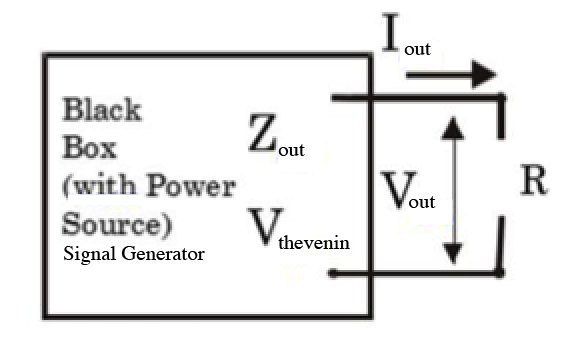
\includegraphics[width=0.5\textwidth]{figure/Z_output_setup}
\caption{The circuit setup used to measure the output impedance of the signal generator.}
\label{Z_output_setup}
\end{figure}

\begin{figure}[h!]
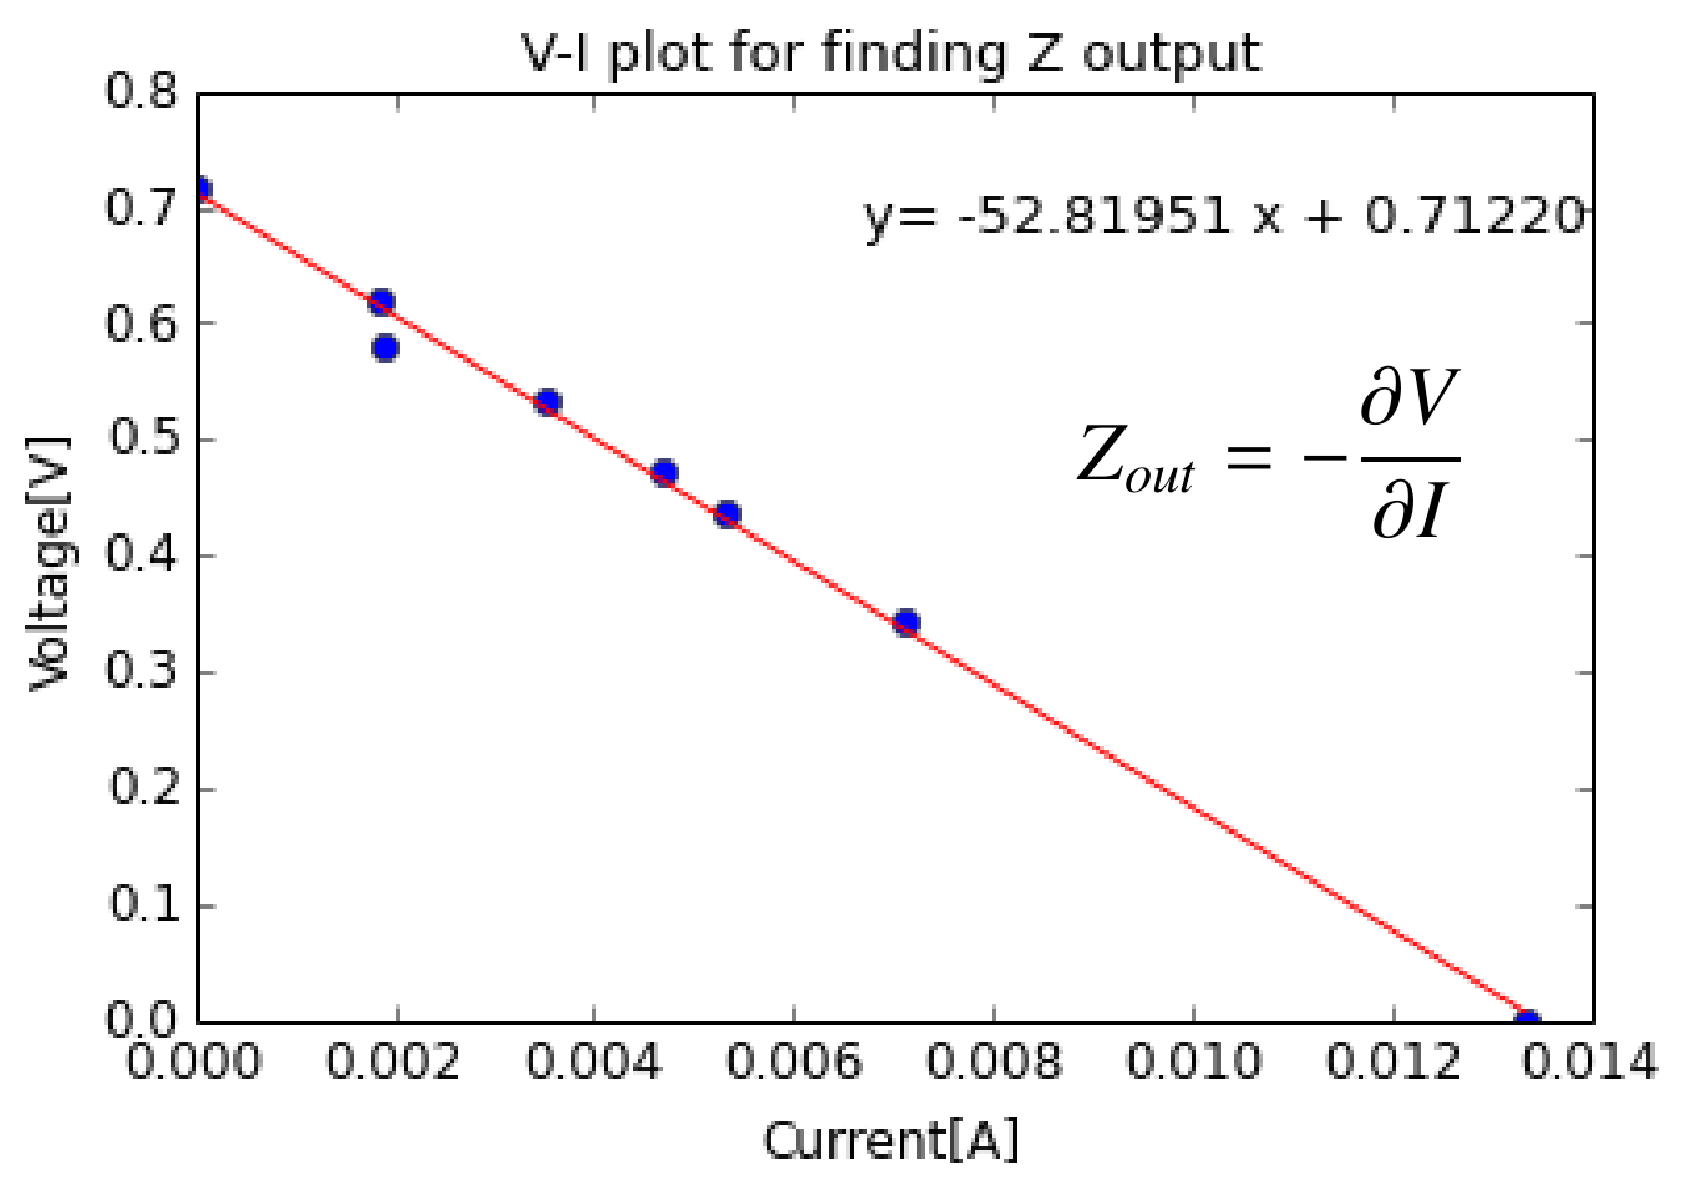
\includegraphics[width=0.5\textwidth]{figure/Z_output_plot}
\caption{The V-I graph for variable resistance 0,47,82,100,330,150,220, $\infty \Omega$, where the slope is the output impedance.}
\label{Z_output_plots}
\end{figure}
We also used a potentiometer to substitute the variable resistance. The initial potential difference across the signal generator at 0$\Omega$ was 0.71515V. When the voltage drops in half, the resistance of the potentiometer is 47.728$\Omega$. Although the potentiometer has the benefit of not having to be removed when we change the resistance, it is hard to achieve the half-voltage point since manual adjustments of the knob tends to over- or under-shoot the exact resistance value.
%%%%%%%%%%%%%%%%%%%%%%%%%%%%%%%%%%%%%%%%%%
\paragraph{\textbf{2.6}}
We set up an RC circuit as shown in Fig. \ref{rc_setup} and vary the frequency from 20Hz to 20kHz
\begin{figure}[h!]
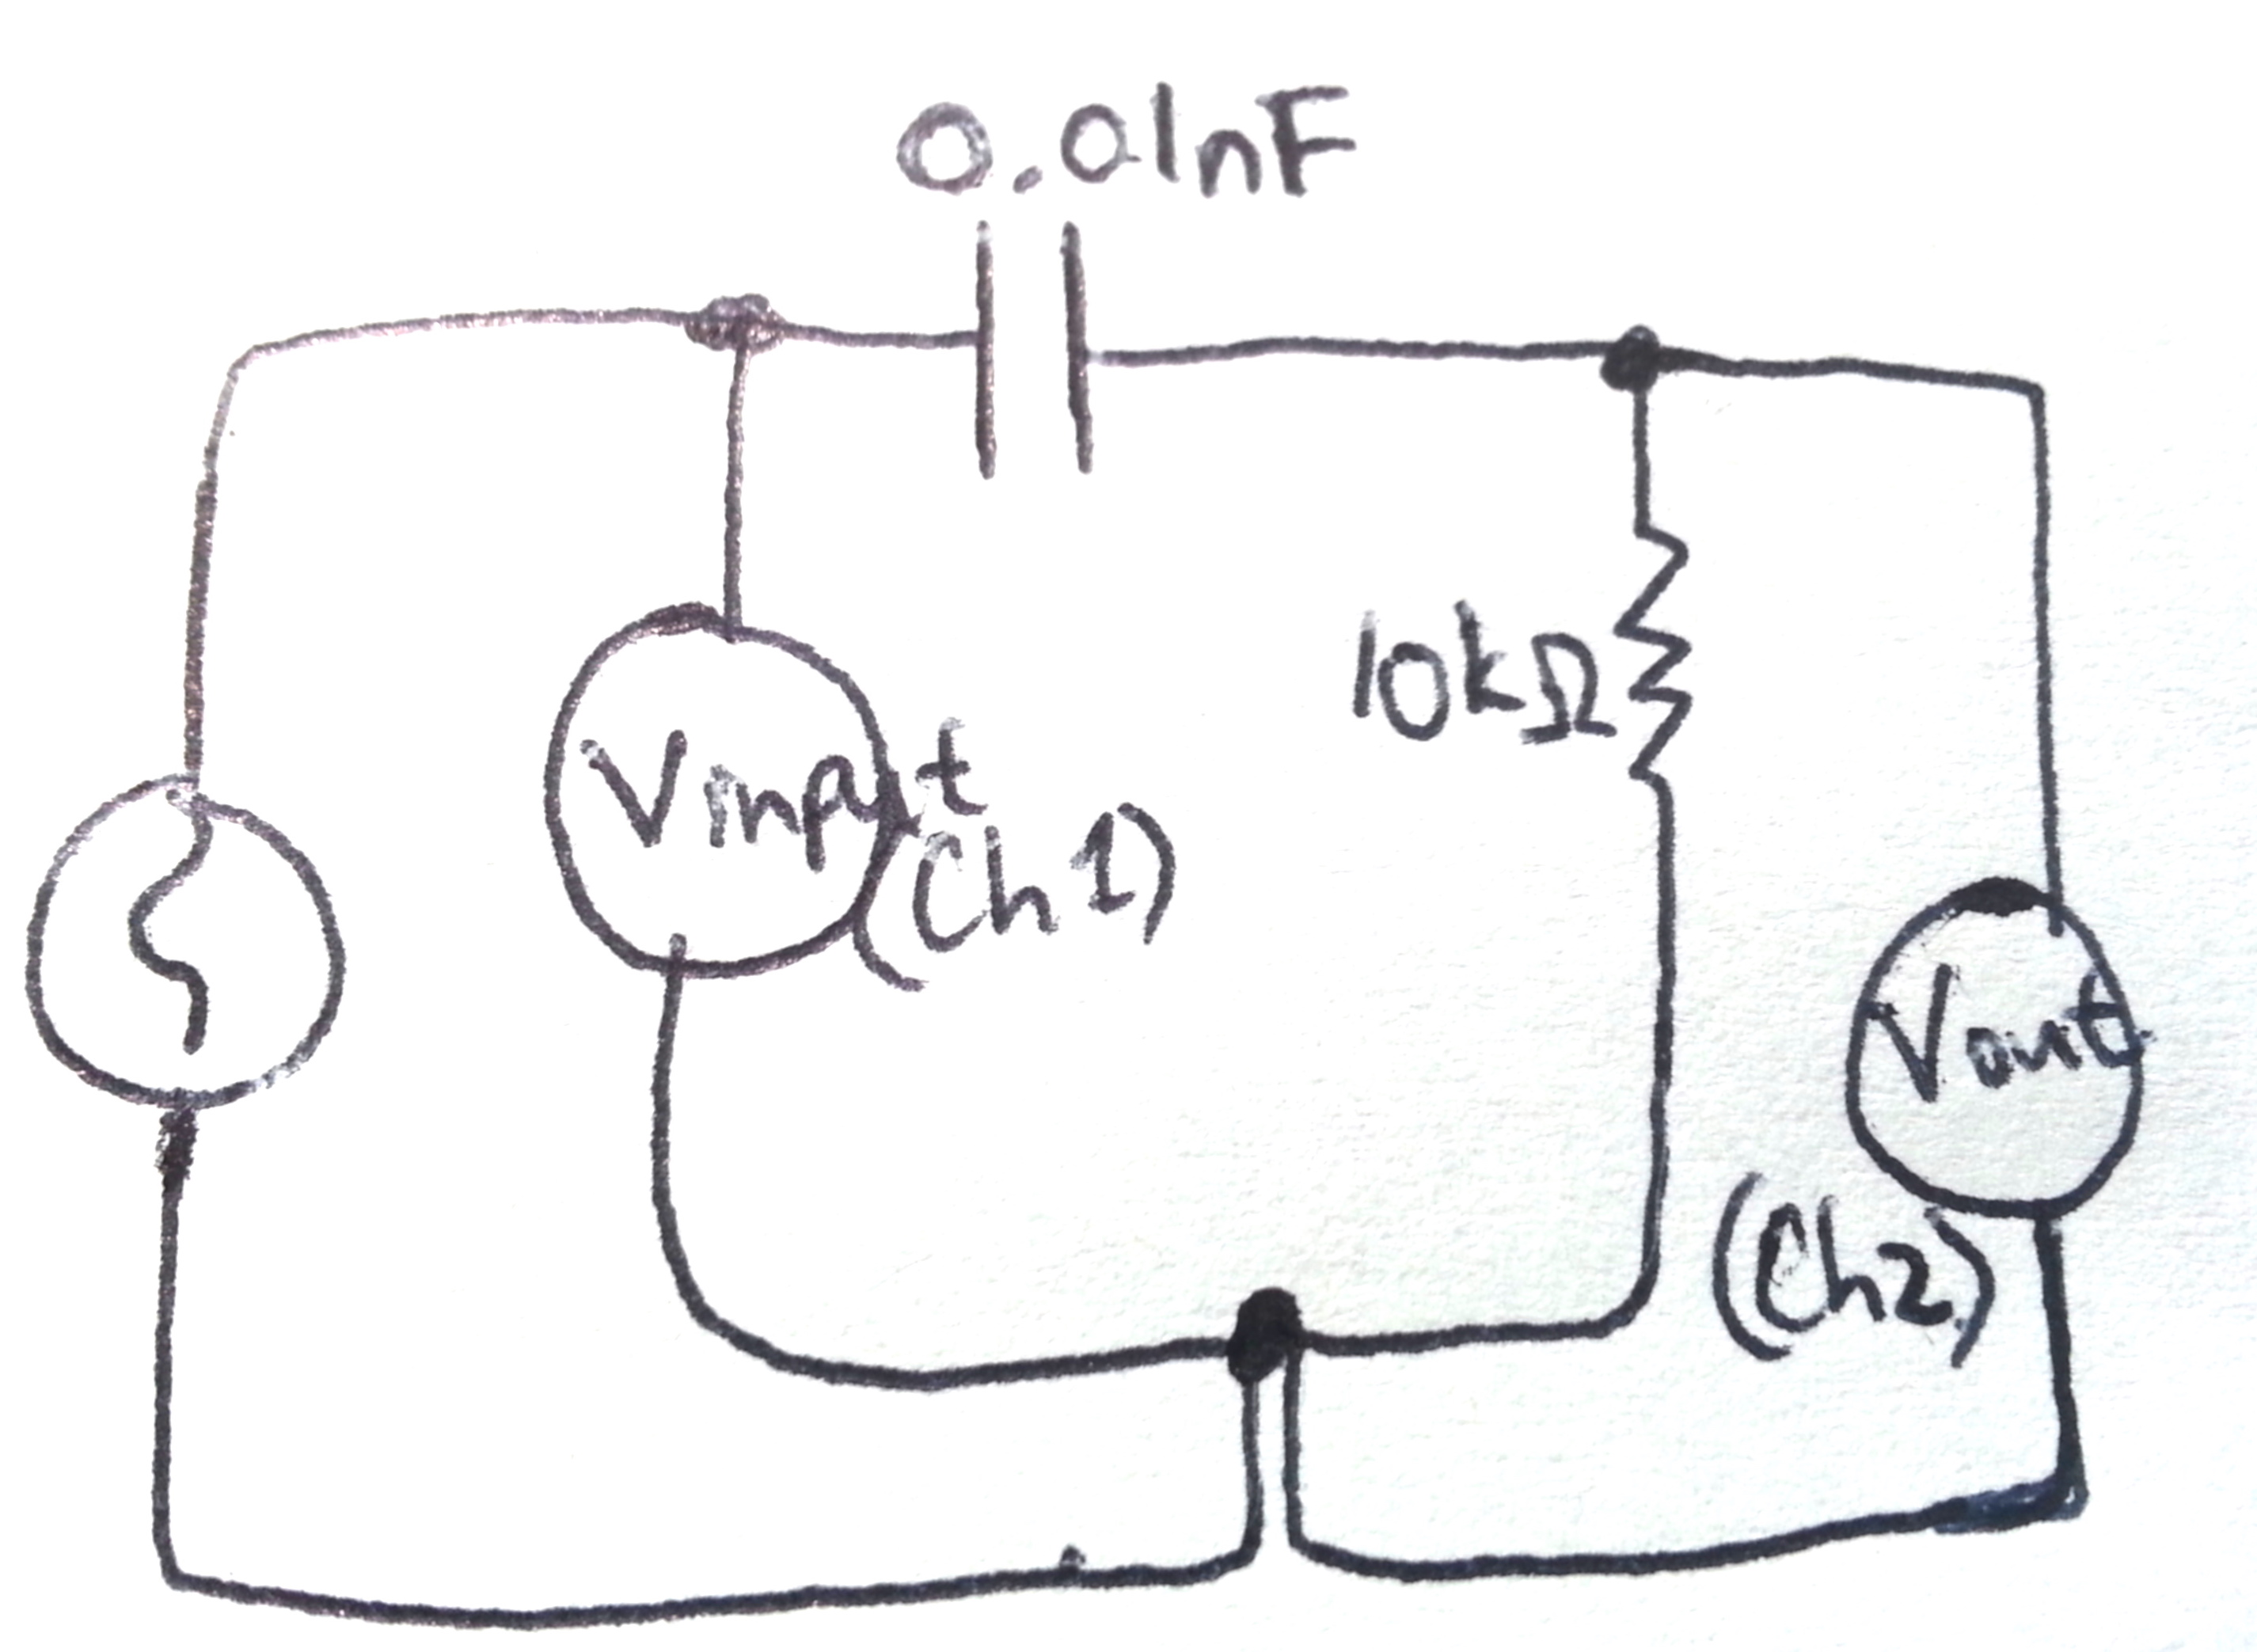
\includegraphics[width=0.5\textwidth]{figure/rc_setup}
\caption{The experimental setup for the RC circuit}
\label{rc_setup}
\end{figure}
We measure the the capacitance and resistance of the 0.01\(\mu F\) capacitor and 100k\(\Omega\) resistor with both the DMM and the LCR meter, and find that they both lie within 10\% of their nominal values. Then, we compute the \(V_{out}/V_{in}\) and plot these against frequency as shown in Fig\ref{rc_circuit}.  We find the location of the roll-off point if we plot the \(y = \frac{1}{\sqrt{2}}\) and estimate that it is located at around 1kHz. The reason why we mark the roll-off point at \(\frac{1}{\sqrt{2}} \) is that this is where transfer function is -3dB (equivalent to a power attenuation by a factor of 2). 
 \begin{figure}[h!]
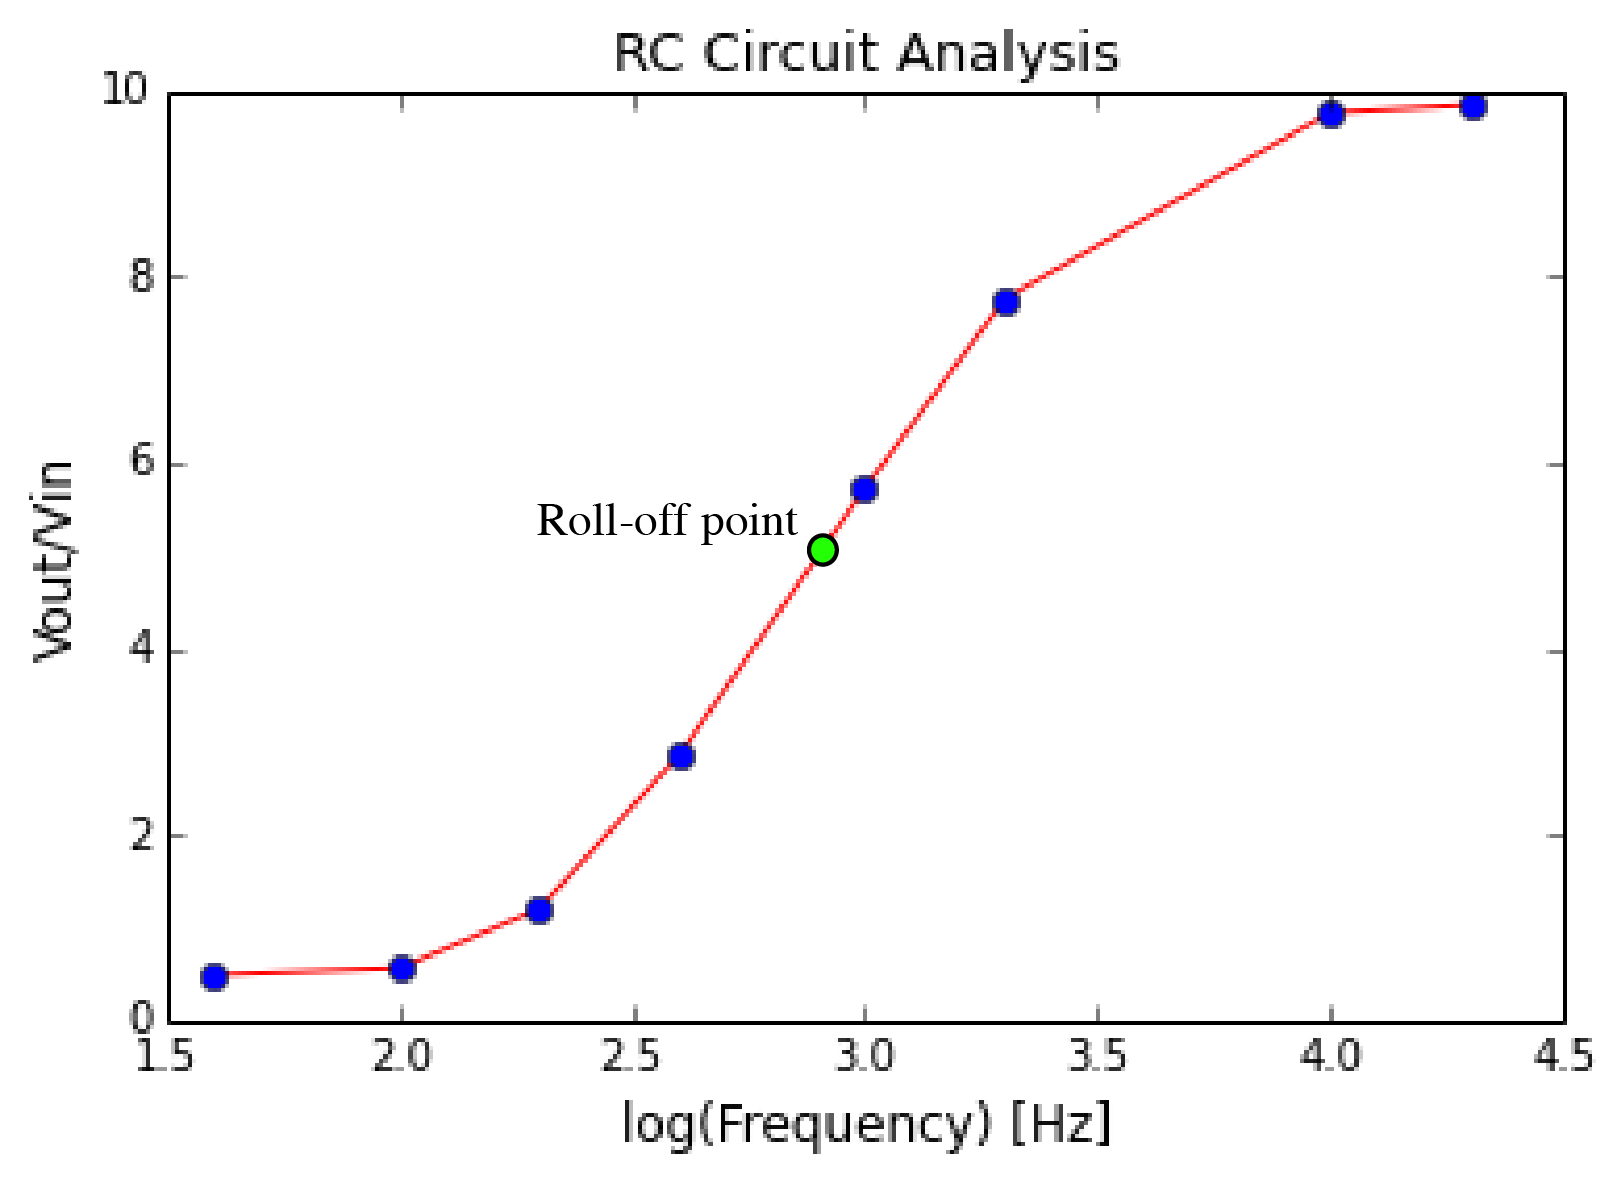
\includegraphics[width=0.5\textwidth]{figure/rc_circuit}
\caption{The ratio of the input and output voltage as we varied frequency, with the green point marking the roll-off point.}
\label{rc_circuit}
\end{figure}
\par We measure the phase between input and output for the 20kHz signal and obtained a phase difference of 5.754\degree, but this value fluctuates with time.
%%%%%%%%%%%%%%%%%%%%%%%%%%%%%%%%%%%%%%%%%%
\paragraph{\textbf{2.7, 2.8}}
We set the time base of the oscilloscope to XY mode, so that the two signals are plotted as an ellipse. Then we center the two signals so that both the X and Y offset is at 0V, to ensure a accurate measure of the intercept and maximum. Using the formula we derived in the Prelab, we can compute the phase shift between signals. \footnote{Even though we used the cursor to find these two readings, the resolution on our chosen X and Y may introduce measurement error in our data.}
\begin{equation}
\delta = \frac{y_{int}}{y_{max}}=\frac{1V}{1.01V}=81.931 \degree
\end{equation}
%%%%%%%%%%%%%%%%%%%%%%%%%%%%%%%%%%%%%%%%%%
\paragraph{\textbf{2.9}}
Using the oscilloscope's ``measurement" option, we take the phase shift reading as we varied the frequency of the input signal, shown in Fig. \ref{phase_plot}.
\begin{figure}[h!]
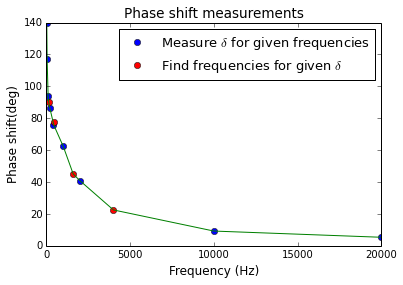
\includegraphics[width=0.5\textwidth]{figure/phase_plot}
\caption{The red data points are obtained by approximating the frequencies that corresponds to $\delta $ =0\degree, 22.5\degree, 77.5\degree, 90\degree  }
\label{phase_plot}
\end{figure}
%%%%%%%%%%%%%%%%%%%%%%%%%%%%%%%%%%%%%%%%%%
\paragraph{\textbf{2.10}}
If the output voltage of a black box decreases by 20\% with a load of 1k$\Omega$, the output impedance of the black box is calculated by:
$$Z_{out} = \frac{V-V_{out}}{I} =\frac{V-0.8V}{0.8V/1k\Omega} $$. 
$$Z_{out} = \frac{0.2V}{0.8V}1000\Omega=250\Omega$$
So the output impedance is 250$\Omega$.
%%%%%%%%%%%%%%%%%%%%%%%%%%%%%%%%%%%%%%%%%%
\paragraph{\textbf{2.11}}
Conventional light bulb is a non linear circuit component since as the bulb lights up, the temperature of the bulb (and therefore the resistors in the circuit) heats up. Due to the temperature-dependence of resistance, the power, current and voltage relation can not be simply described by Ohm's law. We can prove that this is not the case by computing the power output using Ohm's law:
\begin{equation}
P = \frac{V^2}{R} = \frac{(110V)^2}{9\Omega}=1344W
\end{equation}
This is an order of magnitude off from the correct, nominal 100W power number given, therefore Ohm's law does not hold for light bulbs.
%%%%%%%%%%%%%%%%%%%%%%%%%%%%%%%%%%%%%%%%%%
\paragraph{\textbf{2.12}}
The transfer function of a circuit is the ratio of its output and input signal, in units of decibel as: 
\begin{equation}
\frac{P_{out}}{P_{in}} = H = 20 log_{10} \Bigg|\frac{V_{out}}{V_{in}}\Bigg|
\end{equation}
We plot Fig.\ref{bode} using the result we obtained from question 1.2.6's RC circuit.
\begin{figure}[h!]
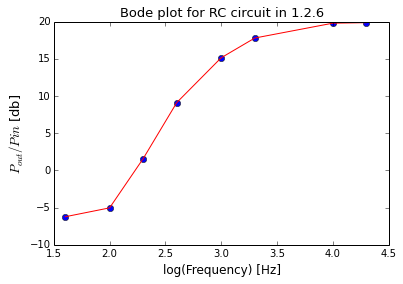
\includegraphics[width=0.5\textwidth]{figure/bode}
\caption{Plotting the transfer function versus log-scaled frequency.}
\label{bode}
\end{figure}
Then we plot the phase shift versus log of the frequency in Fig. \ref{phase2}:
\begin{figure}[h!]
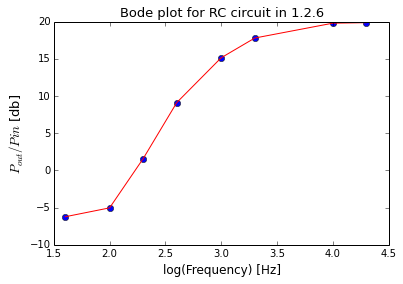
\includegraphics[width=0.5\textwidth]{figure/bode}
\caption{Plotting the phase shift versus log-scaled frequency.}
\label{phase2}
\end{figure}
We then compare the experimental and theoretical curves for the expected transfer function as shown in Fig.\ref{thexp}.
\begin{figure}[h!]
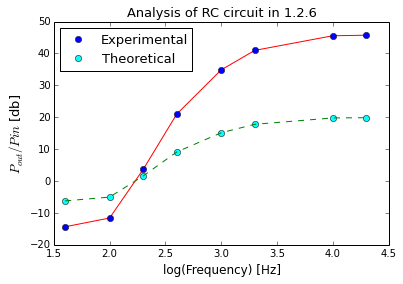
\includegraphics[width=0.5\textwidth]{figure/experiment_theory}
\caption{The experimental and theoretical graphs  shows that the roll off points approximately agree, despite the curves looking quite different near the upper end.}
\label{thexp}
\end{figure}
%%%%%%%%%%%%%%%%%%%%%%%%%%%%%%%%%%%%%%%%%%
\paragraph{\textbf{2.13}}
We send a pulse signal with settings of period=750ns, offset =600mV, amplitude =1.2 V$_{pp}$, delay = 75.00ns, and duty cycle = 4\%. After connecting to the 50$\Omega$ terminator, the amplitude decreased by about a factor of 2, as shown in Fig.\ref{terminator}, to the desirable amplitude of $\approx 1.2V$ . 
\par  Then, we shorted the input signal by connecting a wire between the BNC's inner and outer conductor.  This effectively brings the voltage of the signal and ground to equipotential. Therefore, it brings the signal's voltage to zero, as shown in Fig.\ref{short1}.
\begin{figure}[h!]
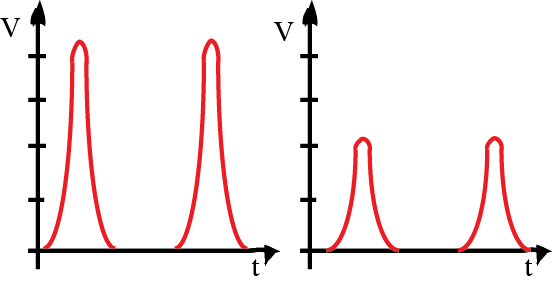
\includegraphics[width=0.5\textwidth]{figure/2_13_50ohmTerminator}
\caption{The ticks on the y axes is 500mV/div. The left figure is the original scope trace and the right figure is the scope trace after connecting to the 50$\Omega$ terminator.}
\label{terminator}
\end{figure}
\begin{figure}[h!]
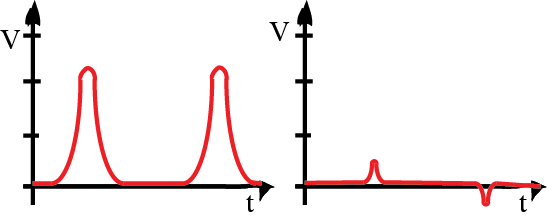
\includegraphics[width=0.5\textwidth]{figure/2_13_short1}
\caption{The ticks on the y axes is 500mV/div. The left figure is the original scope trace and the right figure is the scope trace after shorting the signal with the outer conductor. The amplitude is significantly suppressed and the secondary signal looks reflected.}
\label{short1}
\end{figure}
\begin{figure}[h!]
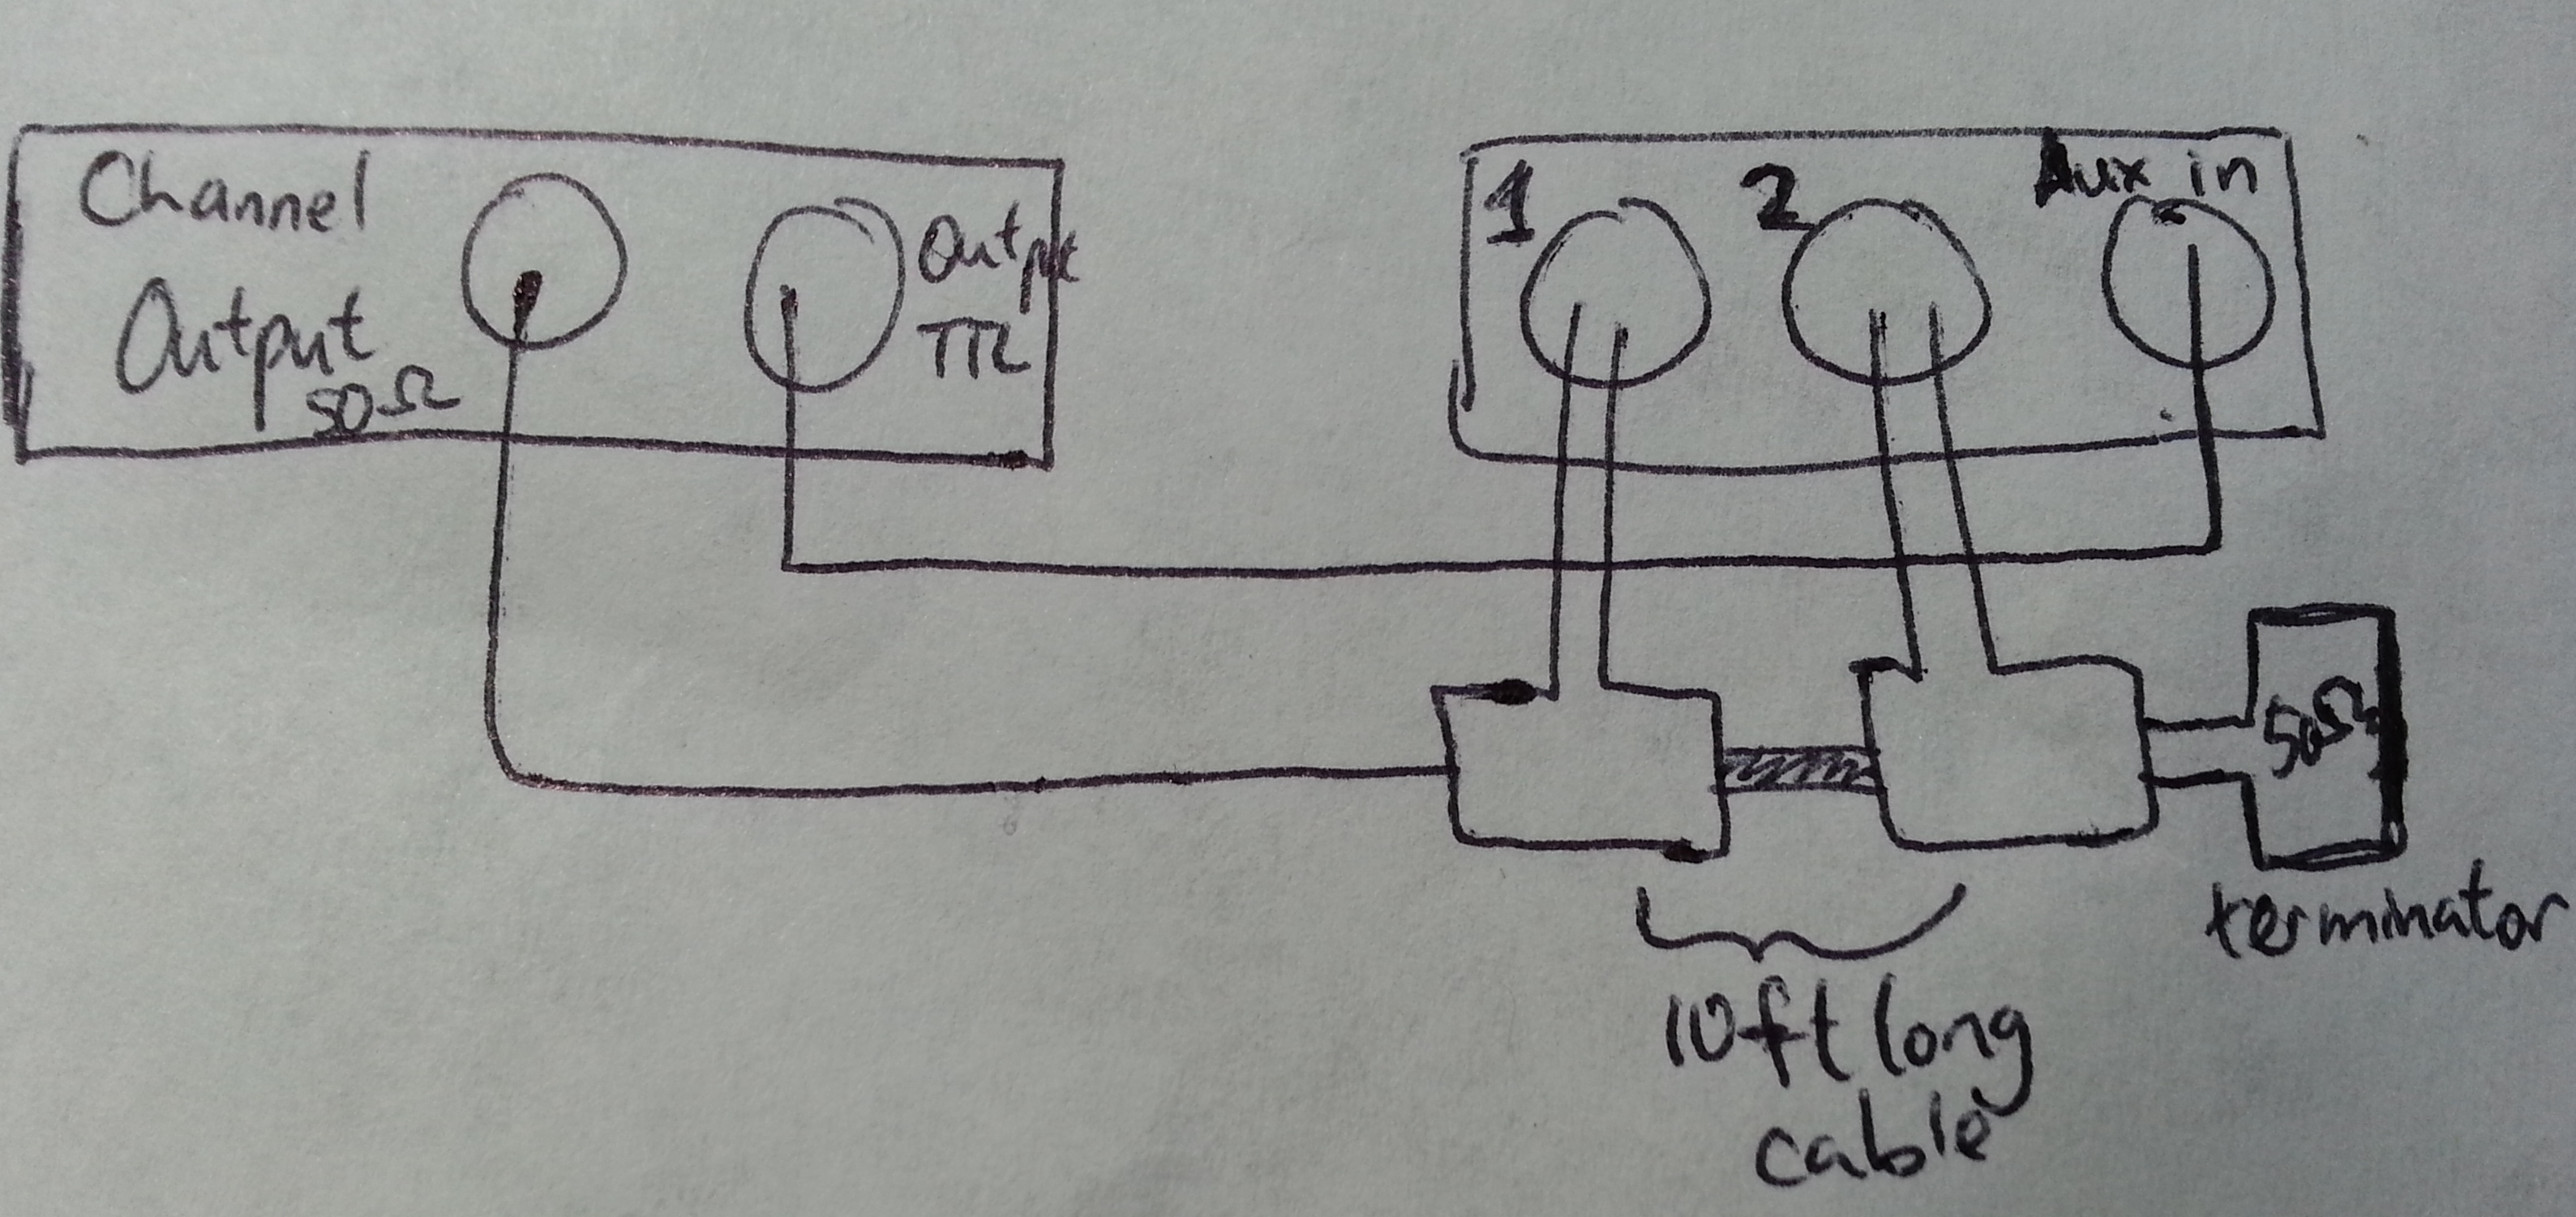
\includegraphics[width=0.5\textwidth]{figure/10ftlongsetup}
\caption{Setup of the signal generator and oscilloscope.}
\label{10ftlongsetup}
\end{figure}
We attached a 10 feet long cable  to the second channel via the Fig. \ref{10ftlongsetup} setup and  detect a time lag between incoming signal from channel 1 and channel 2 as shown in Fig.\ref{timelag1}. 
\begin{figure}[h!]
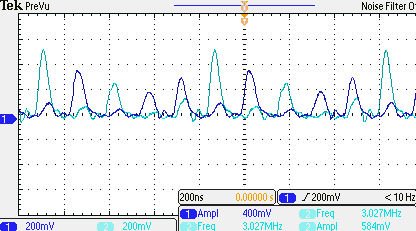
\includegraphics[width=0.5\textwidth]{figure/2_13_timelag_setup}
\caption{By changing the frequency of the signal, the phase difference of the peak maintains but the width of the signal changes. This makes sense because the signal still travels at the same speed and has to traverse the same amount of distance from channel 1 to channel 2 even when the frequency is changed.}
\label{timelag1}
\end{figure}
We again connect the 50$\Omega$ terminator which attenuates the signal. Likewise, we again find that the amplitude of the shorted signal diminishes to zero, as shown in Fig.\ref{shorted2}. By attaching a 200$\Omega$ resistor in series to the output channel, Fig.\ref{2_13_50ohmR} demonstrates that the signal looks more or less the same in shape, but the 2nd channel signal is slightly lower than the first.
\begin{figure}[h!]
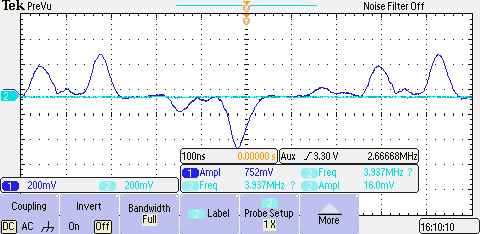
\includegraphics[width=0.5\textwidth]{figure/2_13_shorted}
\caption{While the Channel 2 signal zeroes, some of the signal in Channel 1 is reflected.}
\label{shorted2}
\end{figure}
\begin{figure}[h!]
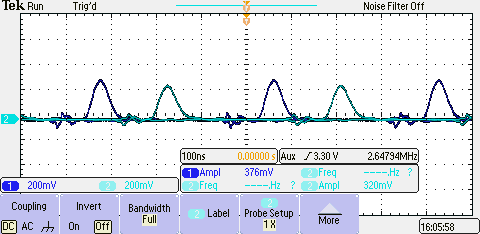
\includegraphics[width=0.5\textwidth]{figure/2_13_50ohmR}
\caption{200$\Omega$ resistor setup.}
\label{2_13_50ohmR}
\end{figure}

%%%%%%%%%%%%%%%%%%%%%%%%%%%%%%%%%%%%%%%%%%
\paragraph{\textbf{2.14}}
\par  If we assume that signals travel at 2/3c, it takes 152 nano seconds for the light to travel from one end the cable to another, as computed by $ t=(30.5 m)/(2/3(3\times10^8  m/s))=152 ns$.
\par The reason we see extra pulses on the A channel is due to the phase shift between the signals. Since we hooked up the scope to itself, we see a reflection pulse travelling opposite to the direction of propagation. The reason the extra pulses are sometimes upright, upside-down, or not there at all depending upon what we put at the end of the coax line, is because of the different indices of refraction of mediums. 
\par Depending on the refraction index, the light bends at an angle which causes a phase shift in the signal that is being read on the oscilloscope's screen. When light travel from a less dense to a denser medium (i.e. the resistor case), some is transmitted and some is reflected with $\lambda$/2 phase shift. In the case where the end is shorted, there is no transmission and the wave is completely reflected with the phase shift. 
%%%%%%%%%%%%%%%%%%%%%%%%%%%%%%%%%%%%%%%%%%
\paragraph{\textbf{2.15}}
We built a bandpass filter with roll-off points at $f_1$=500Hz and $f_2$=10kHz. By choosing impedances such that the first stage is not affected by the loading of the second stage, we wanted most of the voltage drop to occur at the end of the circuit. For the high-pass filter, set 3dB peak to rolloff freuqncy: 
\begin{align*}
500Hz = \frac{1}{2\pi RC}
\\
\frac{1}{RC}=1000\pi Hz = 3141.59Hz
\end{align*}\begin{figure}[h!]
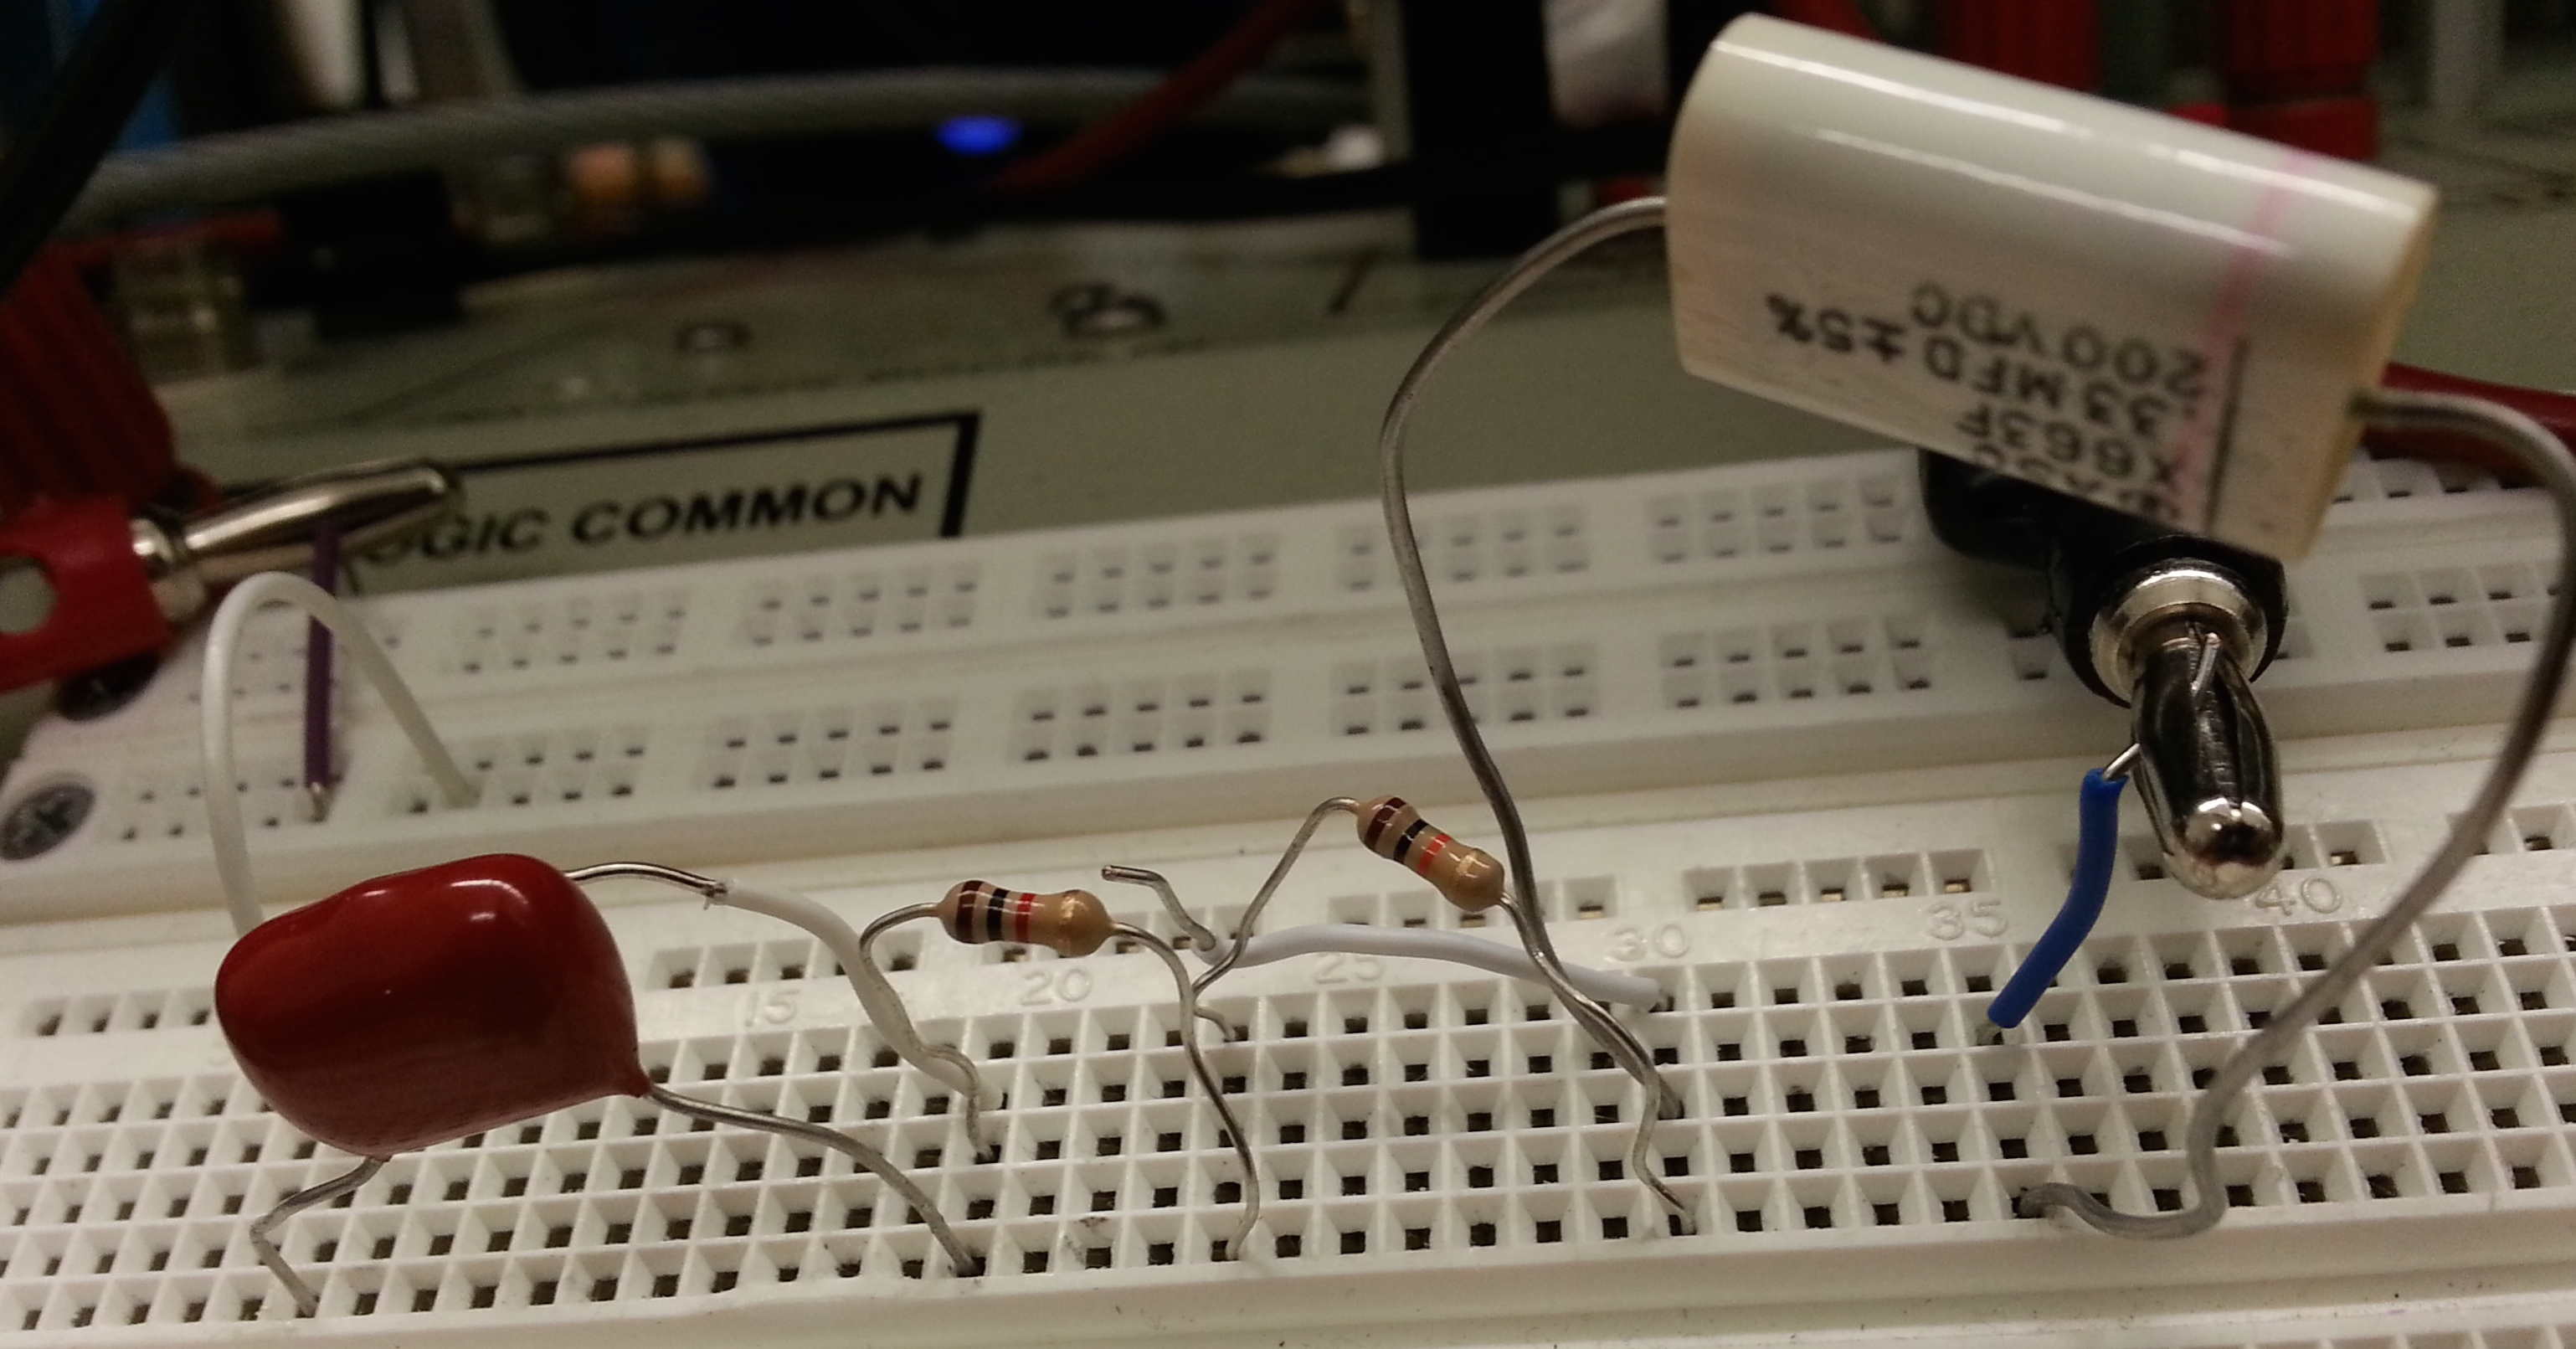
\includegraphics[width=0.5\textwidth]{figure/filter}
\caption{high pass and low pass RC filter}
\label{filter}
\end{figure}
We choose to use a 1k$\Omega$ resistor and 0.33 $\mu F $capacitor. Similarly for the low pass filter, we compute:
\begin{align*}
f_{3db}=10000= \frac{1}{2\pi RC}
\\RC = \frac{1}{20000}=1.59\times10^{-5} \Omega F
\end{align*}
Therefore, we use a 1k$\Omega$ resistor and 0.01 $\mu$ capacitor to build our low pass filter. A schematic of our design is shown in Fig. \ref{schema}.
\begin{figure}[h!]
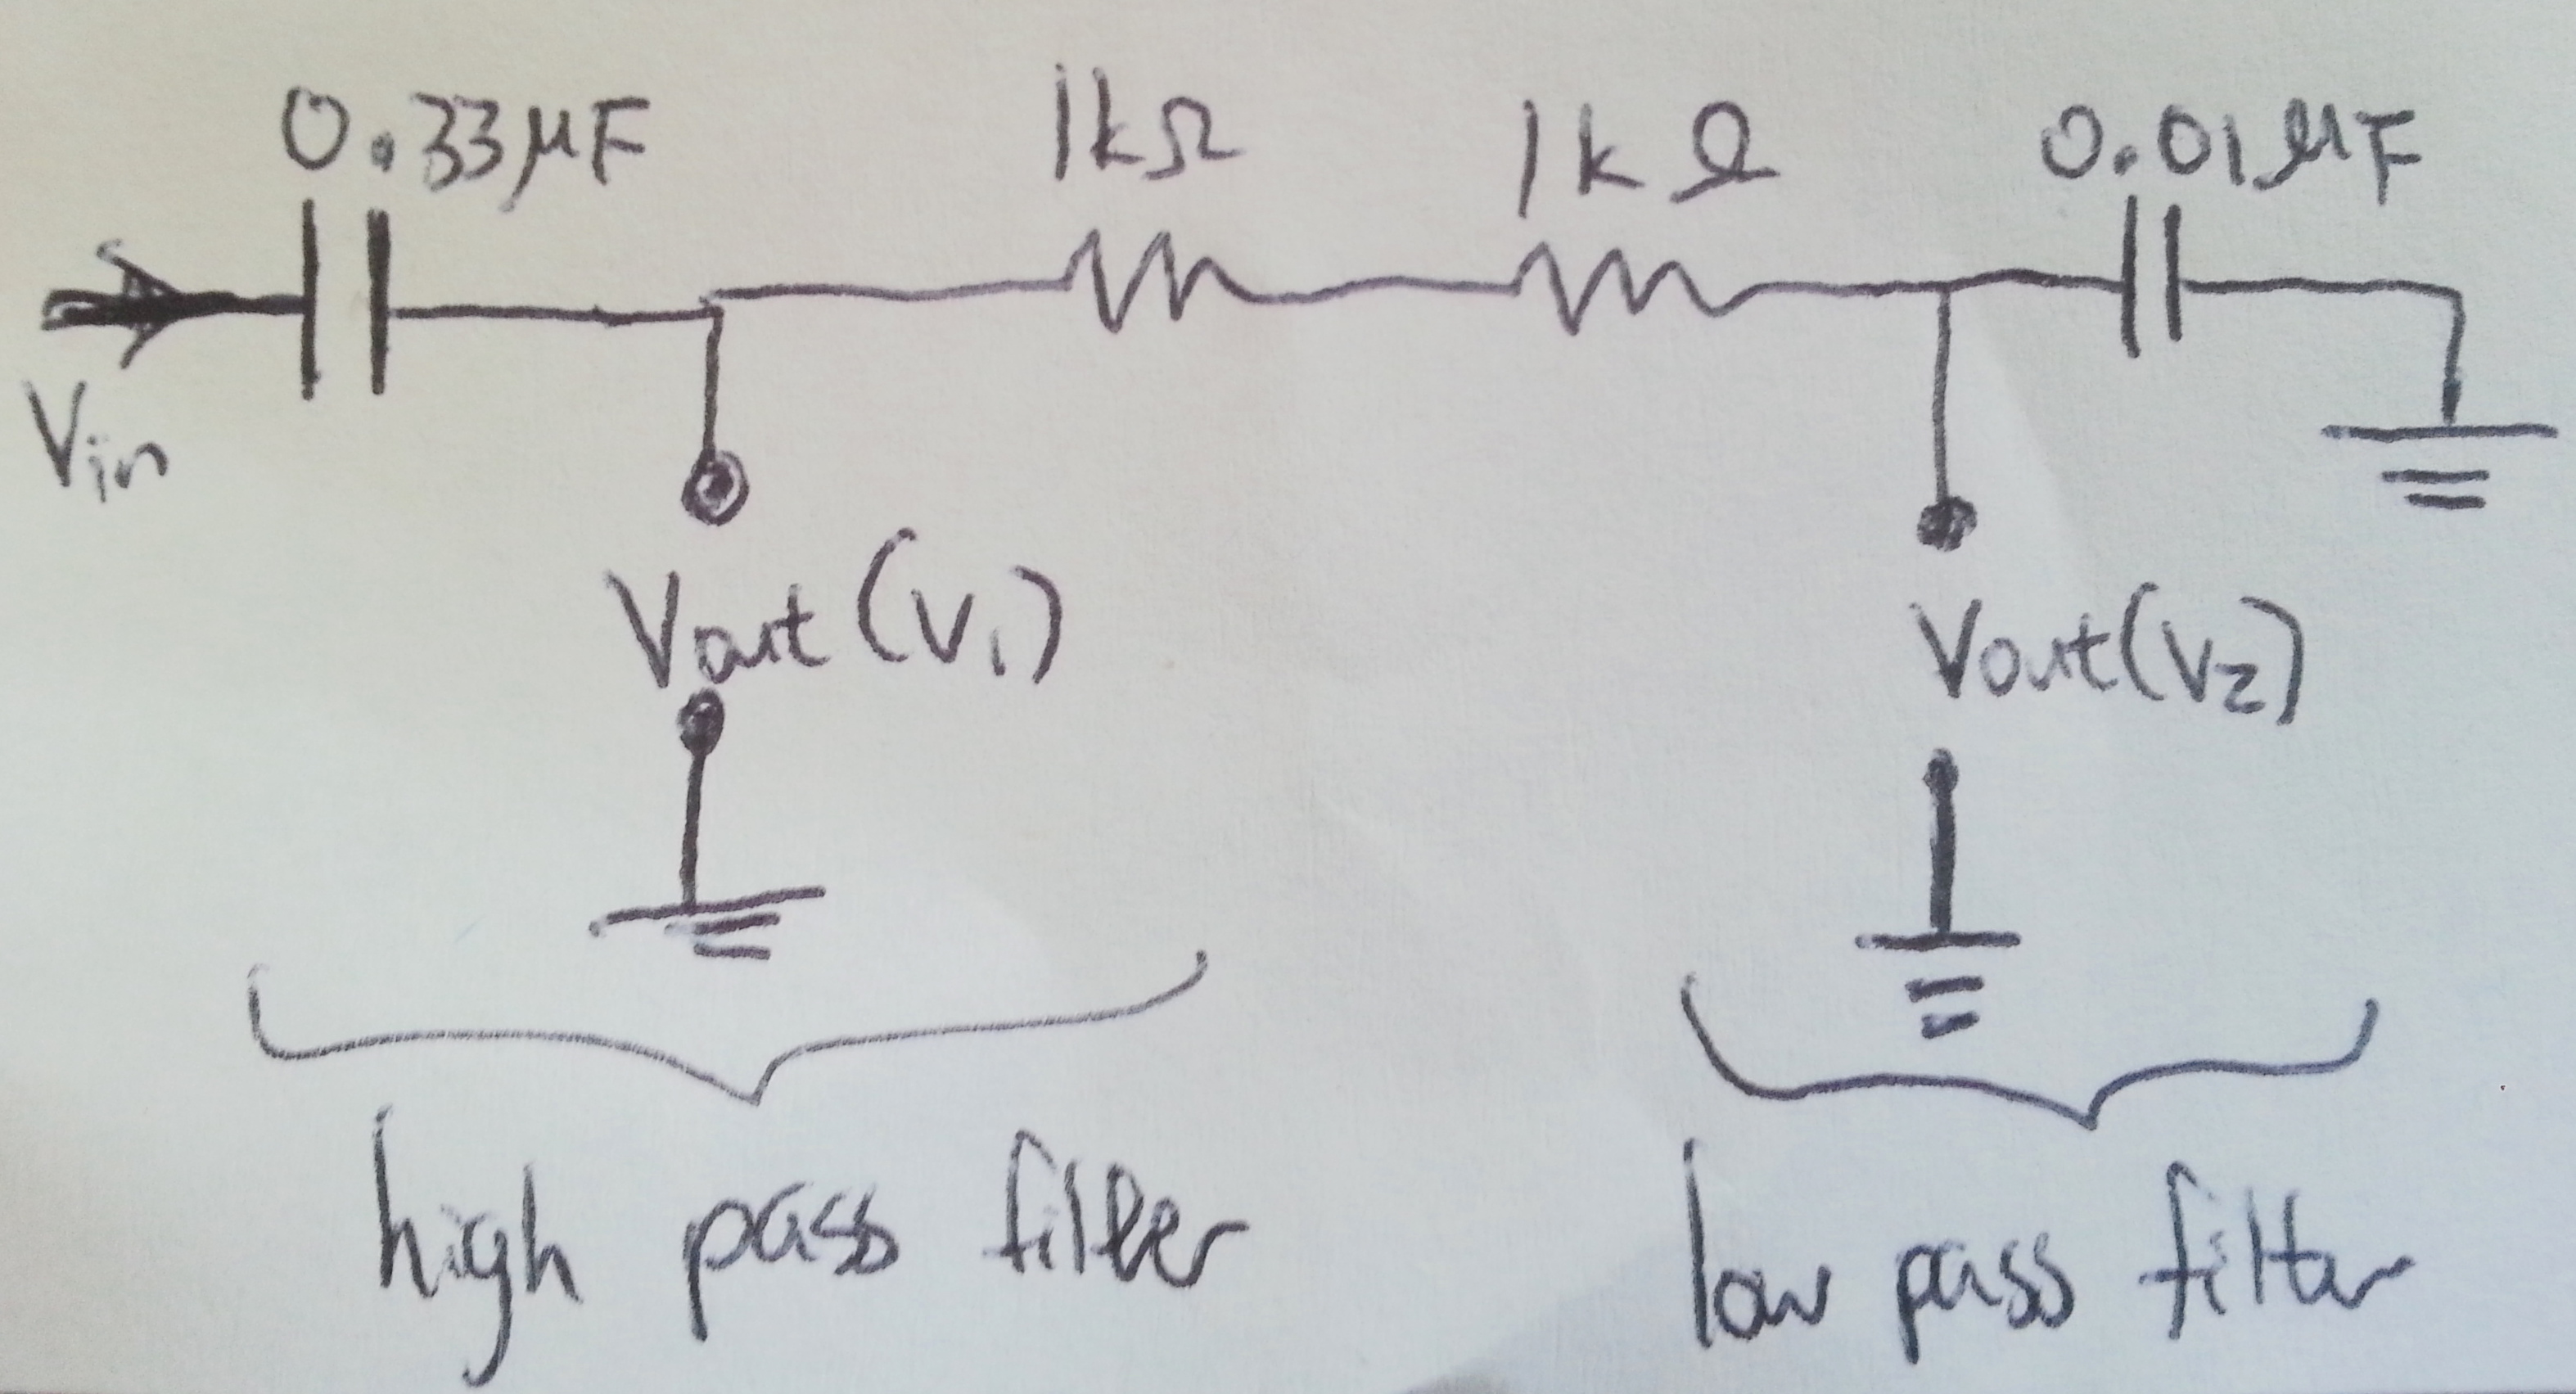
\includegraphics[width=0.5\textwidth]{figure/schema}
\caption{Schematic diagram of high pass and low pass filters.}
\label{schema}
\end{figure}
We test the performance of the filter by passing in signals of different frequencies and then measuring the voltage at $V_1$ and $V_2$ as shown in Fig. \ref{filter_plot}.
\begin{figure}[h!]
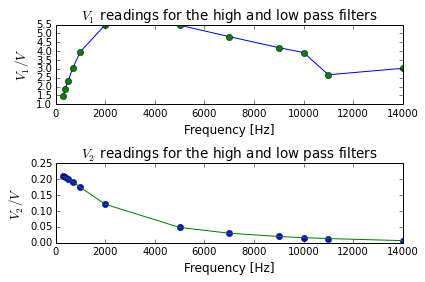
\includegraphics[width=0.5\textwidth]{figure/filter_plot}
\caption{We can see in the top figure that at low frequencies, not a lot of signal is passed through, but as we increased the frequency, more high frequency signals are passed through. Likewise, in the bottom graph, the low pass filter initially lets in lots of the low-frequency signal, but cuts away almost all of the high frequency signal. The difference in absolute magnitude of voltages at $V_1$ and $V_2$ is due to the fact that the signal has to travell through the two 1k$\Omega$ resistors, which decreases the voltage at $V_2$. }
\label{filter_plot}
\end{figure}
 \section{Conclusion}
In this lab, we gained familiarity with using the equipment in BSC lab through hands-on experience with the DMM, breadboard, and oscilloscopes. We practiced reading descriptions in a schematic diagram and its implementations, and applied it to construct linear circuits. Using these linear circuits and other experiments, we explored the physics behind of Thevenin's theorem, filters, \\impedance, and AC circuits. Throughout the whole lab, we conduct basic error analysis on the measurements made by the oscilloscope and other BSC lab instrumentation.
\section*{Acknowledgments}
\begin{footnotesize}
The author would like to acknowledge support from the GSI in this lab and thank my partner, Leah Tom, for helpful discussion and collaboration that helped this work. We also appreciate Sissi Wang for helping us with the oscilloscope settings for question 1.2.7.
\end{footnotesize}
  \section*{References}
 \begin{footnotesize}
 \begin{itemize}
 \item Horowitz, Paul, and Winfield Hill. \textit{The Art of Electronics}. Cambridge: Cambridge UP, 1989. Print.
 \item ``Lab 1 - Introductory Experiments and Linear Circuits I." \textit{Donald A. Glaser Advanced Lab.} Regents of the University of California, n.d. Web. 01 Feb. 2015.
  \item ``Writing Lab Reports." \textit{Donald A. Glaser Advanced Lab.} Regents of the University of California, n.d. Web. 01 Feb. 2015.
% \item Press, William H., and William T. Vetterling. \textit{Numerical Recipes in C: The Art of Scientific Computing}. Cambridge University Press, 1992.  
\end{itemize}
% \bibliography{references}
%\bibliographystyle{elsarticle-harv}
  \end{footnotesize}

\end{document}
